\documentclass[a4paper,12pt]{report}

\usepackage[english, francais]{babel}
\usepackage[utf8]{inputenc}
\usepackage[T1]{fontenc}
%\usepackage{french}
%\usepackage[utf8]{inputenc}
%\usepackage{lmodern}
%\usepackage[francais, english]{babel}
\usepackage{fancyvrb}
\usepackage[pdftex]{graphicx}
\usepackage{setspace}
\usepackage{listings}
\lstset{breaklines=true}
% \usepackage{glossaries}

\usepackage[
%nonumberlist, %do not show page numbers
acronym,      %generate acronym listing
toc,          %show listings as entries in table of contents
section]      %use section level for toc entries
{glossaries}

%\glossarystyle{sublistdotted}
\usepackage[pdftex,
        bookmarks = true,           % Signets
        bookmarksnumbered = true,   % Signets numerotes
	pdfstartview = FitV,        % La page prend toute la hauteur
	colorlinks=true,
	citecolor=black,urlcolor=blue,linkcolor=red,
	pdfauthor={Damien Lambla},
	pdftitle={Maintenance, statistiques et développement à Disneyland Paris},
 	pdfsubject={Rapport de mission},
	plainpages=false,
	pdfpagelabels,
	bookmarks,
	breaklinks=true,
   	hyperindex,
	linktocpage=true]	% pour colorier seulement le numéros dans la TOC	
{hyperref}
% \usepackage{frbib}

\makeglossaries
\pagestyle{empty}
\title{Rapport de mission}
\author{Damien \textsc{Lambla}}


\newcommand{\reporttitle}{Maintenance, statistiques et développement à Disneyland Paris}     % Titre
\newcommand{\reportauthor}{Damien \textsc{Lambla}} % Auteur
\newcommand{\reportsubject}{Rapport de mission} % Sujet
\newcommand{\HRule}{\rule{\linewidth}{0.5mm}}
\setlength{\parskip}{1ex} % Espace entre les paragraphes
\onehalfspacing
\begin{document}
  % Inspiré de http://en.wikibooks.org/wiki/LaTeX/Title_Creation

\begin{titlepage}

\begin{center}

\begin{minipage}[t]{0.48\textwidth}
  \begin{flushleft}
    
\includegraphics [width=30mm]{images/logo-univ.jpg} \\[0.5cm]
    \begin{spacing}{1.5}
      \textsc{\LARGE Université de ...}
    \end{spacing}
  \end{flushleft}
\end{minipage}
\begin{minipage}[t]{0.48\textwidth}
  \begin{flushright}
    
\includegraphics [width=30mm]{images/logo-societe.jpg} \\[0.5cm]
    \textsc{\LARGE Entreprise}
  \end{flushright}
\end{minipage} \\[1.5cm]

\textsc{\Large \reportsubject}\\[0.5cm]
\HRule \\[0.4cm]
{\huge \bfseries \reporttitle}\\[0.4cm]
\HRule \\[1.5cm]

\begin{minipage}[t]{0.3\textwidth}
  \begin{flushleft} \large
    \emph{Auteur :}\\
    \reportauthor
  \end{flushleft}
\end{minipage}
\begin{minipage}[t]{0.6\textwidth}
  \begin{flushright} \large
    \emph{Responsables :} \\
    M.~Jean \textsc{Machin} \\
    M.~Pierre \textsc{Bidon}
  \end{flushright}
\end{minipage}

\vfill

{\large 17 novembre 2011}

\end{center}

\end{titlepage}

  \newpage
   \null
  \newpage
  \cleardoublepage % Dans le cas du recto verso, ajoute une page blanche si besoin
  \tableofcontents % Table des matières
  %manque table des figures
  
  \sloppy          % Justification moins stricte : des mots ne dépasseront pas des paragraphes
  \cleardoublepage
  
  \pagestyle{plain}
  
\setcounter{page}{1} % Réinitialisation du compteur
\pagenumbering{arabic}
  
  \chapter*{Remerciements}
\addcontentsline{toc}{chapter}{Remerciements}

\paragraph{}
Tout d'abord, je tiens à remercier Stéphanie \textsc{Amar}, ma maître d'apprentissage, pour m'avoir accepté dans son équipe.
Je me dois également de remercier Loïc \textsc{Laine}, technico-commercial, et Jacques \textsc{Semoun}, logisticien intégrateur, pour m'avoir aidé lors de mes difficultés. 
Un grand merci également aux techniciens de Spie qui m'ont énormément appris, tant sur l'aspect professionnel que sur l'aspect social d'une entreprise.
\paragraph{}
Je voudrais également exprimer ma gratitude à la grande famille des \foreignlanguage{english}{Cast Members\footnote{Employés de Disneyland}} pour m'avoir invité dans le monde merveilleux de Walt \textsc{Disney}.
\paragraph{}
Un dernier remerciement à M.~Chan \textsc{Leduc}, à M.~Philippe \textsc{Bonnot} ainsi qu'a tous mes professeurs sans qui je n'aurais pas su répondre aux attentes de l'entreprise.
\paragraph{}
\newacronym{cfa}{CFA}{Centre de Formation des Apprentis}
% \newglossaryentry{CFA}{name={CFA},description={Centre de Formation des Apprentis}}
Je n'oublie pas non plus Mme.~Jocelyne \textsc{Capmal}, ainsi que tous les membres du \gls{cfa}\footnote{Centre de Formation des Apprentis} AFIA, qui nous ont aidé, mes camarades et moi, à trouver une entreprise.

% \chapter*{Thanks}
% \addcontentsline{toc}{chapter}{Thanks}

% \paragraph{}
% First, I want to thanks Stéphanie \textsc{Amar}, my internship master, for giving me the chance to be in his team.
% I have to thanks Loïc \textsc{Laine}, a technico-commercial, and Jacques \textsc{Semoun}, the logistics integrator, for help me when I was in troubles.
% Also a big thanks to the entire team of techniciens of Spie who learn me a lots of things, in the professional aspect as well as in the social aspect of an enterprise.
% \paragraph{}
% \newglossaryentry{Cast Members}{name={Cast Members},description={Employés de Disneyland}}
% I want to tell my gratitude to the great family of the \gls{Cast Members} for inviting me in the wonderfull world of Walt \textsc{Disney}.
% \paragraph{}
% A last thanks to M.~Chan \textsc{Leduc}, and M.~Philippe \textsc{Bonnot}, and to all my teachers without who I couldn't answer to the expectations of the company.
% \paragraph{}
% I don't forget Mme.~Jocelyne \textsc{Capmal}, and all the members of the \gls{CFA} AFIA which help us, my comrade and me, to find out a company.

  \cleardoublepage
  \chapter*{}
\addcontentsline{toc}{chapter}{Résumé}

\section*{{\huge Résumé}}
\paragraph{}
Mon apprentissage s'est déroulé à Disneyland Paris. Ma mission principale consistait à assurer la maintenance du parc informatique. Lors des deux premières semaines, j'ai pris le temps d'apprendre comment réparer le matériel, puis j'ai été capable d'effectuer des interventions sur site.
Il m'a ensuite été demandé de développer des macros-commandes ainsi qu'un outil d'aide à la planification. Pour cela j'ai dû faire preuve de beaucoup d'autonomie, et de persévérance. Étant le seul développeur de l'équipe, j'ai dû concevoir et mettre en place des solutions pour répondre aux besoins de l'équipe et de mon maître d'apprentissage.


\section*{{\huge Summary}}

\paragraph{}
My internship took place at Disneyland Paris. my principal mission consisted to ensure the maintenance of the informatique park. During the first two weeks, I took the time to learn how to fix the equipment, then I have been capable of doing interventions on the place.
Then, I have been in charge of the developpement of macros-commands and a tool for helping to the planification. For this, I had to show independence and tenacity. I was the only one developper of the team. I had to design and put in place solutions for answer to the needs of the team and to my internship master.

  \cleardoublepage
  \section*{Introduction}
\addcontentsline{toc}{section}{Introduction}

Cet article est d�stin� � favoriser la prise en main de gEDA, suite libre de Conception �lectronique Assist� par Ordinateur.
Ce n'est en aucun cas une documentation suffisante, il a pour but de compl�ter les articles r�dig�s par les concepteurs.

Nous verrons �galement de quel mani�re programmer les PIC (microcontr�leurs de chez Microchip) sous Linux en C. 

Finalement nous �tudierons les cartes �lectroniques permettant la mesure d'une temp�rature avec les sondes Pt100.

 

  \cleardoublepage
  \chapter{Présentation de l'entreprise et des missions}
% \chapter{Présentation de l'entreprise}

% \section{Fondateurs}
% \section{Structure juridique}
% \section{Son développement}
% \section{Ses objectifs}
% \section{Ses clients potentiels}
% \section{Les membres}
% \section{Le lieu}

Dans cette partie, on examinera dans un premier temps l'entreprise afin de situer dans quel contexte j'ai effectué mon année en apprentissage. Puis, je décrirais quelles ont été les différentes missions que j'ai effectué, et j'expliquerais pourquoi elles m'ont été demandées.

%mieux vaut un plan en entonnoir
%les clients, les objectifs de l'entreprise, le fondateur, le rachat par spie, les deux parties (infogérance et ...), 
\section{Présentation de l'entreprise}
\subsection{Une société de services}
\paragraph{}
\newacronym{ssii}{SSII}{Société de Services en Ingénierie Informatique}
\newglossaryentry{cloud}{name={cloud computing},description={Concept qui consiste à déporter sur des serveurs distants des stockages et des traitements informatiques traditionnellement localisés sur des serveurs locaux. cf. \url{http://fr.wikipedia.org/wiki/Cloud_computing}}}
\newglossaryentry{infogerance}{name={infogérance},description={C’est l’externalisation de tout ou partie de la gestion et de l’exploitation du SI à un prestataire informatique tiers (SSII). cf. \url{http://fr.wikipedia.org/wiki/Infogérance}}}
APX est une \gls{ssii} fondée par Noël \textsc{Saille}. Son siège social est situé à Saint Cloud (92). Mais, je dépend du centre de services de Rungis (94).
APX est divisée en deux parties : APX Intégration, et APX \Gls{infogerance}.
La première partie est centrée sur le \foreignlanguage{english}{\gls{cloud}}\footnote{Concept qui consiste à déporter sur des serveurs distants des stockages et des traitements informatiques traditionnellement localisés sur des serveurs locaux. cf. \url{http://fr.wikipedia.org/wiki/Cloud_computing}} : elle aide des clients à migrer ses données sur le \foreignlanguage{english}{cloud}.
Tandis que la deuxième partie est plus axée sur le support et la maintenance en vue de répondre à un besoin d'externalisation des entreprises. La partie infogérance (uniquement) a récemment été rachetée par Spie, une autre \gls{ssii}. Je ne mentionnerais donc que Spie dans ce rapport.
J'ai effectué mes missions dans le domaine de l'\gls{infogerance}\footnote{C’est l’externalisation de tout ou partie de la gestion et de l’exploitation du SI à un prestataire informatique tiers (SSII). cf. \url{http://fr.wikipedia.org/wiki/Infogérance}}.
\subparagraph{}
L'un des plus gros contrats d'infogérance de Spie est celui de Disneyland. Je vais donc vous parler de ce client dans la partie qui suit.


\subsection{Un client}
\paragraph{}
Après avoir exprimé une volonté de changement, Disneyland Paris a confié à Spie la maintenance de son parc informatique, auparavant géré par Econocom (une autre \gls{ssii}).
Depuis septembre 2012, c'est donc Spie qui a repris le contrat de Disneyland Paris.
Disneyland ne sous-traite que la partie maintenance et support technique de son service informatique (pour des raisons financières et des raisons de productivité). Spie ne s'occupe donc pas de la partie \foreignlanguage{english}{hotline} et web.
J'ai donc effectué mes missions au sein des locaux de Spie mis à disposition par Disneyland. Ces locaux sont divisés en trois parties : le stock, les bureaux, et l'atelier.
\subparagraph{}
Après vous avoir parlé de la société dans laquelle j'ai évolué, je vais maintenant décrire l'équipe \textbf{avec}, mais aussi \textbf{pour} laquelle, j'ai travaillé.




\subsection{Une équipe}
\paragraph{}

\newacronym{ot}{OT}{Ordres de Travail}
%\newglossaryentry{ot}{name={OT},description={Ordres de Travail}}
\newglossaryentry{dispatcher}{name={dispatcher},description={Personne chargée de recevoir et retransmettre les \gls{ot}}}
Dans la figure~\ref{organigrammeAPX} page~\pageref{organigrammeAPX}, je décris comment l'équipe est organisée.
J'ai travaillé dans une équipe d'environ 20 membres (cf. fig.~\ref{organigrammeAPX}), composée de techniciens de proximité, de techniciens référents, d'une \foreignlanguage{english}{\gls{team}}, d'un logisticien, d'un logisticien intégrateur, et d'un \foreignlanguage{english}{\gls{dispatcher}\footnote{Personne chargée de recevoir et retransmettre les \gls{ot}}}. Le \foreignlanguage{english}{\gls{team}} gère l'équipe de techniciens. Le logisticien gère le stock de matériels informatiques, et le logisticien intégrateur gère les devis d'installations et les factures de réparations (dans le cas ou le matériel n'est plus réparable par nos propres moyens). Il n'y a donc aucun autre développeur dans l'équipe. Seul le logisticien intégrateur possède des compétences en \gls{vba}.
\paragraph{}
\begin{center}
  \begin{figure}[ht]
    \caption{\label{organigrammeAPX} Organigramme de l'équipe}
    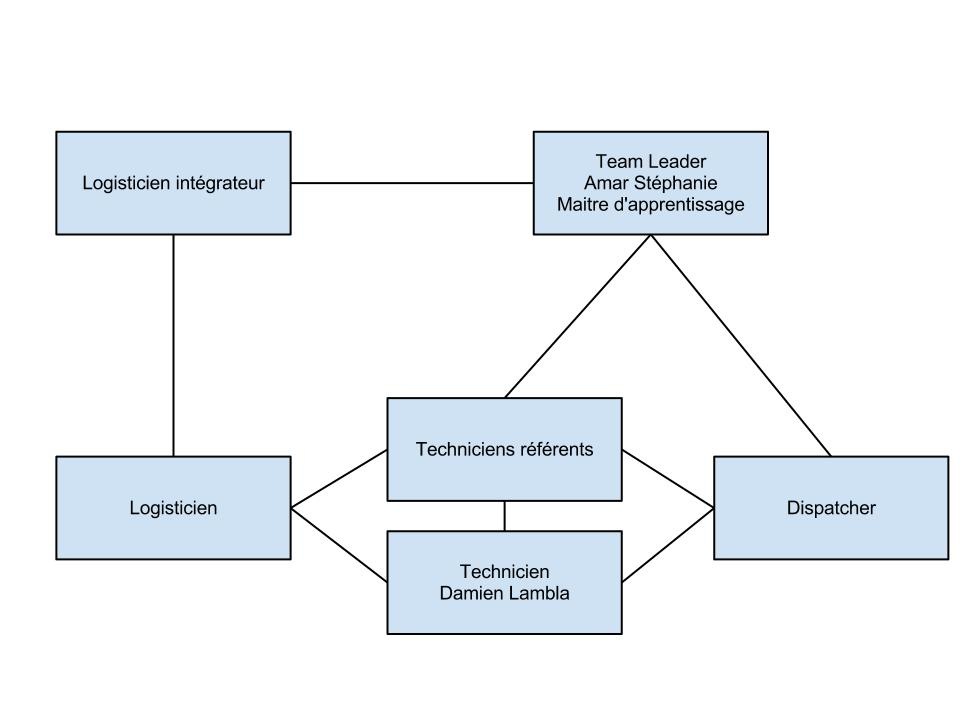
\includegraphics [width=1\textwidth]{images/Organigramme_APX.jpg}
  \end{figure}
\end{center}

  \cleardoublepage
  \section{Présentation des missions}
% \chapter{Description des missions}

\subsection{La maintenance à Disneyland}%maintenance
\paragraph{}
\newacronym{sm7}{SM7}{\foreignlanguage{english}{Serice Manager version 7}}
Ma première mission consistait à appuyer les techniciens en cas de grand nombre d'interventions. Chaque intervention est soumise à des délais. Cela consistait à réceptionner un \gls{ot}\footnote{Ordres de Travail} par fax (et via le logiciel propriétaire \gls{sm7} dont je vous parlerais dans la partie "développement" de ce rapport) et de se rendre sur le lieu de l'intervention avec le matériel adéquat. Ces \gls{ot} sont envoyés par la \foreignlanguage{english}{hotline}. La nature des interventions peut variée. Cela va du simple changement de souris sur un PC\footnote{\foreignlanguage{english}{Personal Computer}} de bureau (dans le \Gls{back office}), à la "remasterisation" d'une caisse récupérée sur le parc. J'assurais donc un soutien aux techniciens durant les périodes de \foreignlanguage{english}{rush}, le plus souvent pendant les vacances scolaires.
\subparagraph{}
Cette première mission à occupé une place importante de mon apprentissage. En effet, j'effectuais ponctuellement des interventions, tout au long de l'année. Je vais maintenant vous parler de ma deuxième mission.


\subsection{Rapports d'intervention et statistiques}%rapport/stat des interventions
\newglossaryentry{macros}{name={macros-commandes},description={Enregistrement des actions effectuées par un utilisateur, au clavier et à la souris, afin de pouvoir les rejouer dans le même ordre automatiquement par la suite. cf. \url{http://fr.wikipedia.org/wiki/Macro-commande}}}
\newglossaryentry{backlog}{name={\foreignlanguage{english}{backlog}},description={Nombre d'incidents non résolus à la fin de la journée}}
\paragraph{}
Par la suite, j'ai appris le \gls{vba} et commencé à développer des \gls{macros}\footnote{Enregistrement des actions effectuées par un utilisateur, au clavier et à la souris, afin de pouvoir les rejouer dans le même ordre automatiquement par la suite. cf. \url{http://fr.wikipedia.org/wiki/Macro-commande}} dans le but d'établir un rapport sur la productivité des techniciens. Je devais traiter des informations extraites du logiciel propriétaire (sous forme d'un tableau Excel) et automatiser des calculs sur ces données après les avoir préalablement traitées. Puis, ce rapport est envoyé au centre de services à Rungis. J'ai ensuite rempli un tableau de bord pour visualiser les données calculées sur une année. 
Ce tableau de bord ne devait pas être recréé : je devais le compléter sans effacer certaines données (comme le \gls{backlog}\footnote{Nombre d'incidents non résolus à la fin de la journée}). 
Ce tableau de bord était rempli manuellement par la \gls{team}.%\foreignlanguage{english}{team leader}.
\subparagraph{}
Cette partie de mon apprentissage m'a permis de mettre à l'épreuve mes connaissances algorithmiques. J'ai ensuite continué le développement avec une mission qui a mobilisé une grande partie de mes compétences informatiques.



\subsection{Développement d'un outil de gestion d'emplois du temps}%emploi du temps
\paragraph{}
Enfin, ma dernière mission consistait à développer un outil de gestion d'emplois du temps permettant à la \foreignlanguage{english}{team leader} de mettre à jour les emplois du temps des techniciens à n’importe quel moment. Lors d'une mise à jour d'un emploi du temps, tout le monde devait en être informé en temps réel. De plus, cela devait permettre une supervision du nombre d'heures travaillées. Les emplois du temps devaient être consultables par les techniciens, selon la semaine ou le trigramme choisis. La liste des techniciens présents devait pouvoir être extraite pour chaque jour. Un système de permissions restreignant les droits de modifications devait être mis en place.

  \cleardoublepage
  % \chapter{Maintenance}
\chapter{Description des missions}

Dans cette partie je détaillerais avec le plus de précisions possibles les missions que j'ai effectuées. C'est pourquoi j'ai choisi d'examiner chaque missions dans une partie. 

\section{Maintenance}

\subsection{L'organisation de Disneyland}%POS,GFS,Bureautique, les delais, les fax, les SLA ...
\paragraph{}
Un découpage de Disneyland à été établi lors de la création du premier contrat entre la société de service qui s'est occupée de la maintenance du parc et Disneyland.
Ce découpage sert à définir des délais de réparation, mais aussi à simplifier la gestion du stock. En effet, chaque matériel et chaque lieu de Disneyland est affecté à un domaine. Ainsi lorsqu'un problème matériel est déclaré, le technicien sait de quelle délai il dispose pour résoudre le problème.

\newacronym{pos}{POS}{\foreignlanguage{english}{Point Of Sell}}
\newacronym{gfs}{GFS}{Gest Facing System}
\paragraph{}
Il y a trois domaines : \gls{pos}, \gls{gfs}(ou \foreignlanguage{english}{Ticketing}) et Bureautique.
Selon la période de l'année et l'affluence des visiteurs, les délais sont plus ou moins courts.
Le domaine \gls{pos} correspond à tout ce qui touche à la vente de produits dérivés et de consommables. C'est un domaine très important pour la rentabilité du parc. Cependant, d'un point de vu maintenance, ce domaine n'est pas le plus important.
En effet, le domaine \gls{gfs} importe beaucoup plus. Il correspond à tout ce qui à un impact direct avec le visiteur. Par exemple les tourniquets d'entrée du parc, ou les décors font partis de ce domaine. C'est le domaine le plus critique. Il a le délais le plus court. Si un tourniquet reste bloqué à l'entrée du parc, le visiteur sera directement touché. 
Enfin, il y a le domaine bureautique. Ce domaine impact quasiment exclusivement les employés de Disneyland. Il correspond au matériel des employés, comme les imprimantes, les ordinateurs, etc. Il s'agit donc du domaine le moins critique. Nous avons entre 8 et 6 heures pour dépanner le matériel du domaine bureautique.

\paragraph{}
Lorsqu'un employé constate un problème technique sur le matériel, il contact la \foreignlanguage{english}{hotline} et demande un numéro d'intervention. La \foreignlanguage{english}{hotline} de son côté crée un \gls{ot} et l'envoie au service concerné par le problème.
S'il s'agit d'un problème électrique, l'\gls{ot} est transmis à la maintenance électrique, s'il s'agit d'un problème réseau, l'\gls{ot} est transmis à la maintenance réseau, etc...
Notre service s'occupe de la maintenance \gls{hardware}. Tout les \gls{ot} nous sont transmis de deux manières : par fax et via \gls{sm7}. cf. figure~\ref{sm7ListeOt} page~\pageref{sm7ListeOt}.
\begin{center}
  \begin{figure}[ht]
    \caption{\label{sm7ListeOt} SM7}
    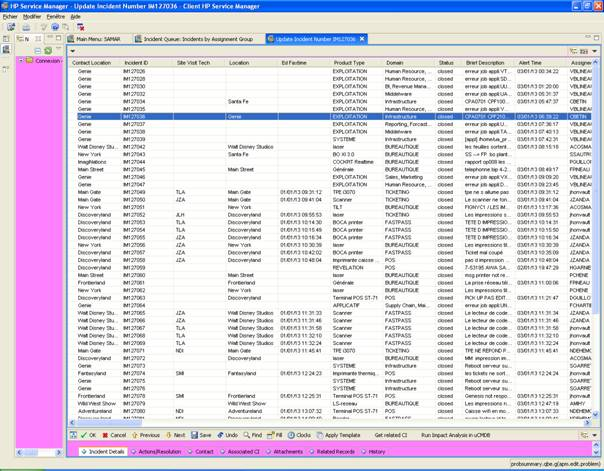
\includegraphics [width=1\textwidth]{images/sm7ListeOt.jpg}
  \end{figure}
\end{center}
Examinons maintenant la façon dont est géré cette \gls{ot} en interne.

\subsection{L'organisation de Spie à Disneyland}%dispatcher, stock, la chef, ...
\paragraph{}
Un fois le fax et l'\gls{ot} reçu, le \gls{dispatcher} effectue un contre-appel afin de s'assurer de la présence de la personne qui a appelé mais aussi pour tenter une réparation par téléphone. Le \gls{dispatcher} peut également prendre des rendez-vous dans le cas où la personne n'est pas disponible dans l’immédiat.
Le \gls{dispatcher} peut alors préparer le matériel dont aura besoin le technicien. Si le matériel doit être changé, alors une sortie de stock doit être effectuée en notant le type de matériel, son ID Disney ainsi que son domaine. Le matériel peut être testé, si le matériel est conditionné. Enfin l'\gls{ot} est assigné à un technicien en fonction du lieu d'intervention et de l'endroit où il se trouve. En effet, si le technicien est déjà en intervention, alors des interventions proches lui seront assignées. 
J'ai pu, durant de courtes périodes, effectuer le travail de \gls{dispatcher}.
Enfin lorsque du matériel revient de réparation, un reparamétrage ou une remasterisation est souvent nécessaire avant de retourner dans le stock. Une intervention en atelier est donc réalisée.
J'ai souvent effectué ce travail en atelier.

Je vais maintenant vous parler de l'intervention sur le terrain de manière plus technique.


\subsection{Le déroulement d'une intervention}%le depart du technicien, le client,...
\paragraph{}
Lorsqu'un technicien débute sa journée, des \gls{ot} lui sont remis sous forme de fax. Après avoir préparé et vérifié son matériel, il part sur le lieu d'intervention en voiture ( même dans les coulisses du parc ). 
Le technicien peut alors réparer le matériel sur place ou bien l'emporter en atelier si nécessaire.

La figure~\ref{st71} page~\pageref{st71} représente une caisse électronique en cours de remasterisation dans l'atelier. Cette remasterisation est une opération très courante, elle résout de nombreux problèmes. J'ai choisi de vous montrer cette réparation comme un exemple car il y a un très grand nombre de matériel différent et donc de problèmes et de solutions différentes. 
Une remasterisation consiste à remettre un "master" (ou un ghost) c'est à dire remettre une image d'un système sur le disque dur d'une caisse. Pour cela on utilise Norton Ghost, sur une clé USB bootable. Ces caisse ne peuvent booter \textbf{que} sur une certaine clé préparé par l'équipe "Customer".
Une fois l'opération terminée, d'autres paramétrages doivent être réalisés, comme par exemple l’ajout d'un pare-feu, l'ajout de certificats pour le wifi, le paramétrage des tiroirs caisse, etc.
\begin{center}
  \begin{figure}[ht]
    \caption{\label{st71} Caisse (ST71) en cours de remasterisation}
    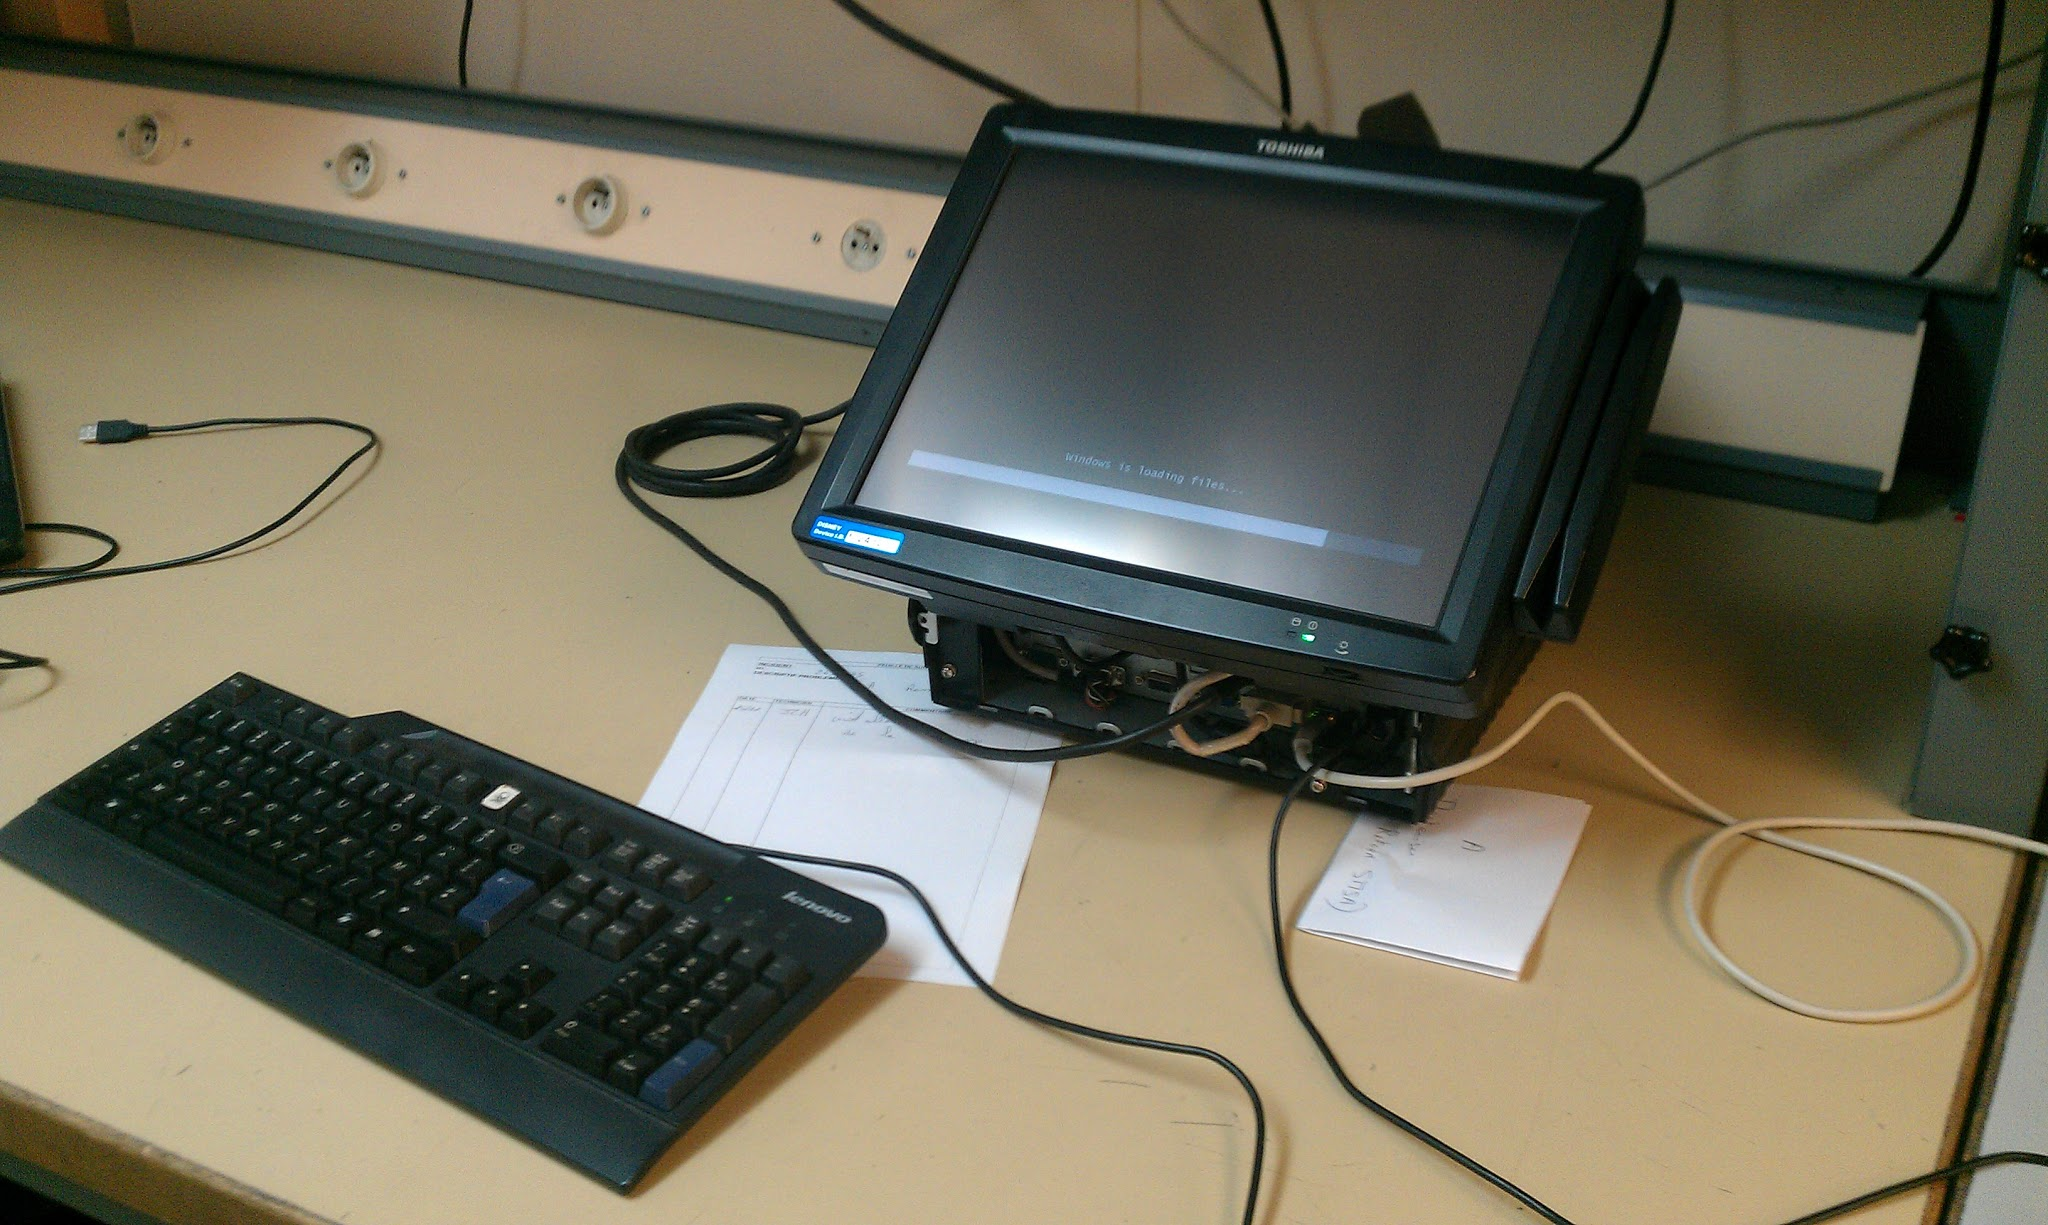
\includegraphics [width=1\textwidth]{images/st71.jpg}
  \end{figure}
\end{center}
\newacronym{ri}{RI}{Rapport d'Intervention}
A la fin d'une intervention, le technicien doit remplir un \gls{ri}, et le faire signer par l'utilisateur du matériel. Ainsi il peut donner le \gls{ri} au \gls{dispatcher} pour clore l'incident. C'est le \gls{dispatcher} qui est chargé de clore les intervention afin que les techniciens gagne du temps.
Pour clore une intervention, le \gls{dispatcher} rempli les champs nécessaires dans \gls{sm7}, et transmet le \gls{ri} au client (Disneyland) après l'avoir scanné et archivé.

  \cleardoublepage
  % \chapter{Macro-commandes}
\section{Macro-commandes}

\subsection{Les différentes macros}%
\paragraph{}
Avant de pouvoir créer une macro \gls{vba} j'ai du apprendre les bases de ce langage et les outils utilisés. Pour cela je me suis aidé de certains sites internet tels que \url{http://www.excel-pratique.com}. J'ai finalement appris tout en créant ma première macro. 

En ce qui concerne les outils utilisés : j'utilisais Excel version 2007 sur Windows XP. La version d'Excel est important car des macros créés sous Excel 2007 ne peuvent pas forcément être lancées sur une version antérieure. 

Je vais maintenant vous parler des macros qui m'ont été demandées. Tout d'abord, il m'a été demandé de créer des macros afin d'automatiser des traitements effectués tous les jours, pour certains, par ma maître d'apprentissage. 

La première macro qui m'a été demandée consistait à calculer des statistiques sur les interventions effectuées par les techniciens. Cette macro a servi de feuille de contrôle des statistiques et des \gls{ri} transmis à la hotline.

Puis, j'ai dû créer une macro servant à éditer un fichier contenant des statistiques sur la productivité de chaque techniciens (cf. figure~\ref{prodDesTech} page~\pageref{prodDesTech}).
\begin{center}
  \begin{figure}[ht]
    \caption{\label{prodDesTech} Tableau de productivité des techniciens}
    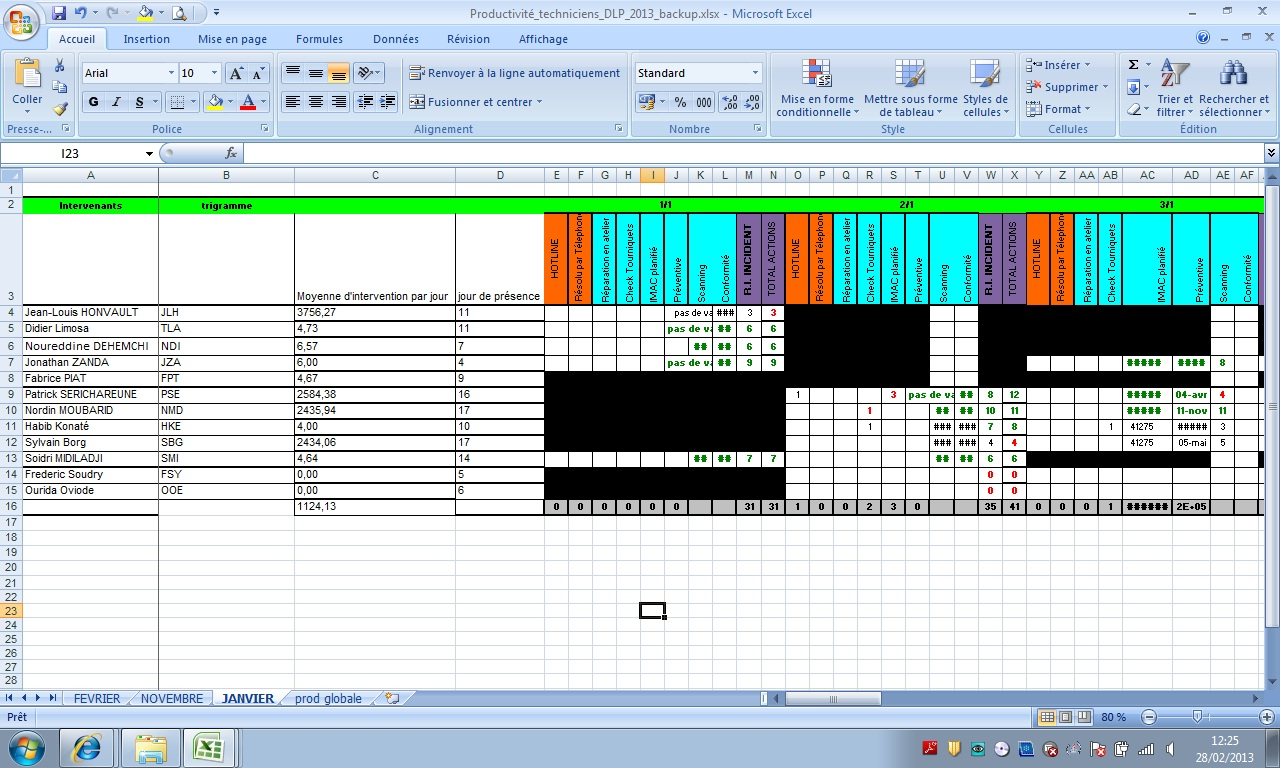
\includegraphics [width=1\textwidth]{images/prodDesTech.jpg}
  \end{figure}
\end{center}
\newacronym{sla}{SLA}{Service Level Agreement}
Ma troisième macro devait elle aussi servir à éditer un fichier déjà existant afin cette fois-ci d'établir un graphique sur le respect des \gls{sla} et des délais de manière plus globale.

Enfin, il m'a été demandé d'extraire automatiquement les listes des interventions résolues puis une deuxième liste pour les interventions en \gls{backlog} (cf. figure~\ref{listeResolu} page~\pageref{listeResolu}). et figure~\ref{listeBacklog} page~\pageref{listeBacklog}. 
Le fichier des interventions en \gls{backlog} doit absolument être édité et non pas recréé. Sinon, il perd tout son intérêt.
\begin{center}
  \begin{figure}[ht]
    \caption{\label{listeResolu} Listes des interventions résolues sur une période donnée}
    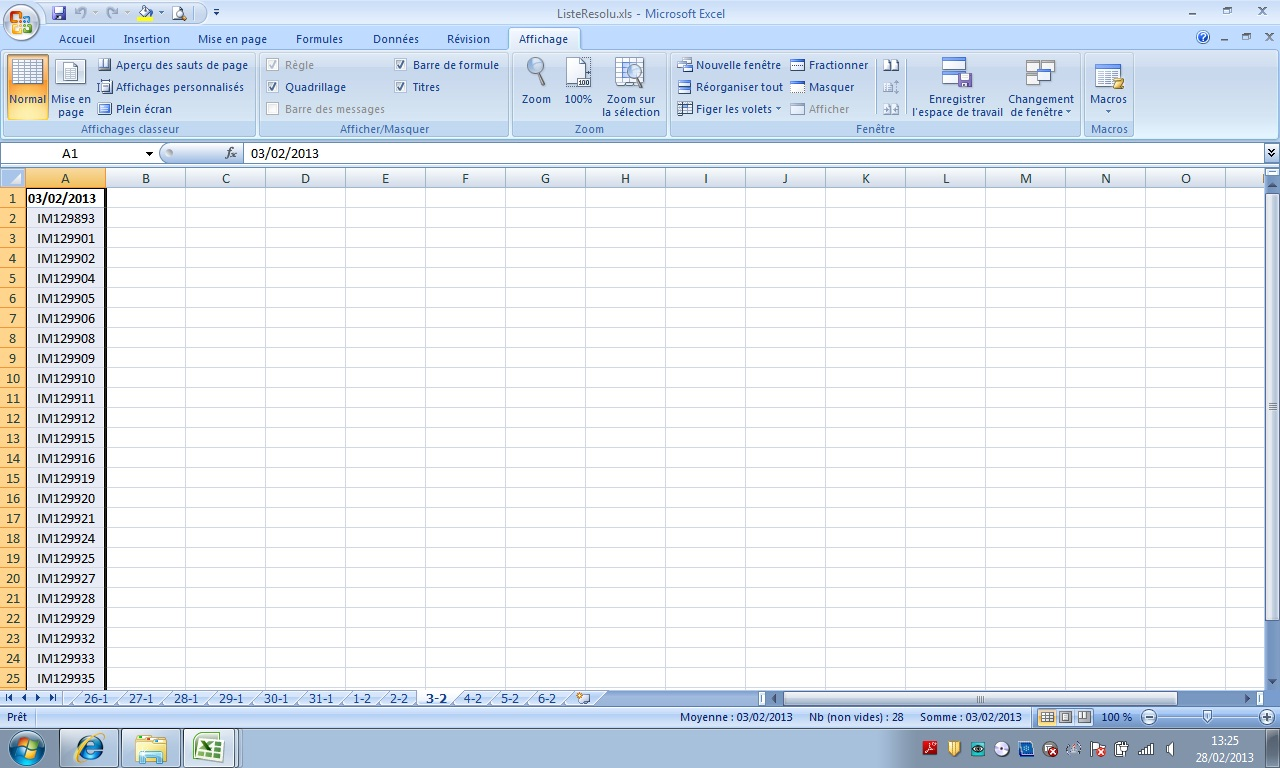
\includegraphics [width=1\textwidth]{images/listeResolu.jpg}
  \end{figure}
\end{center}
\begin{center}
  \begin{figure}[ht]
    \caption{\label{listeBacklog} Listes des interventions en backlog}
    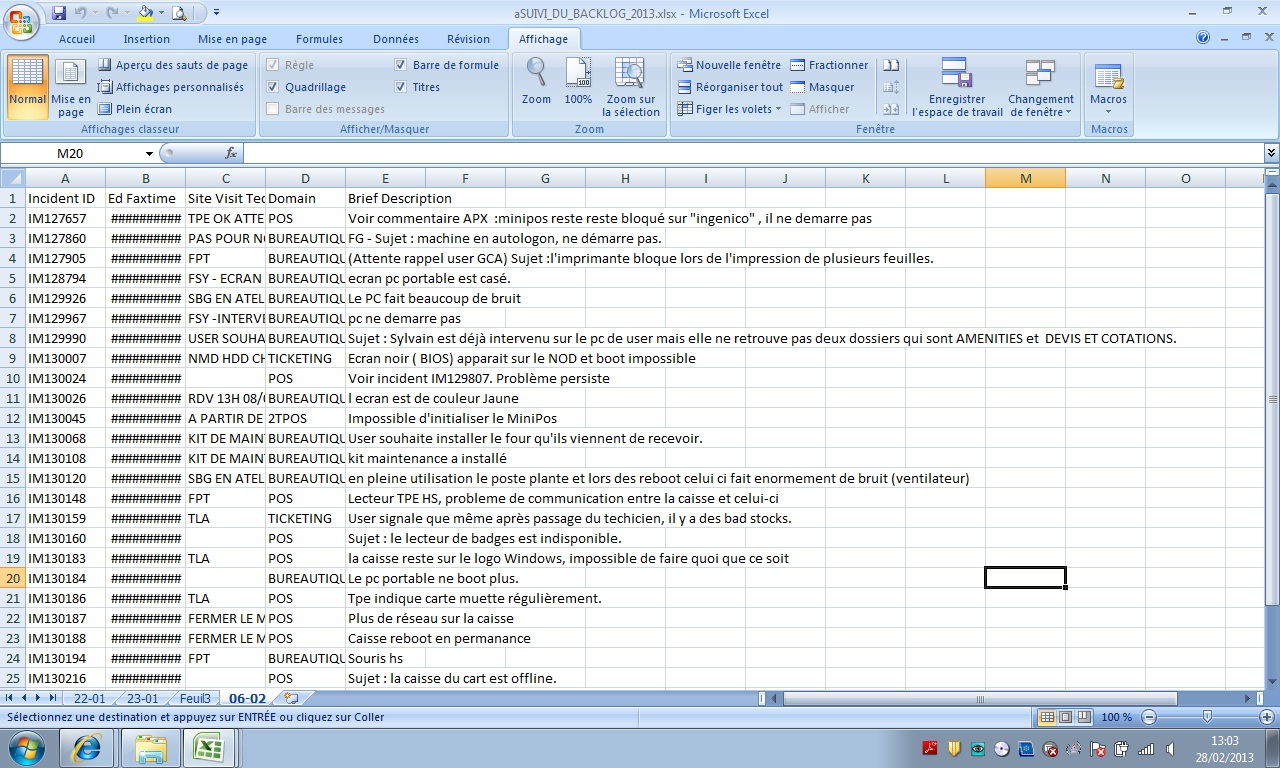
\includegraphics [width=1\textwidth]{images/listeBacklog.jpg}
  \end{figure}
\end{center}


\subsection{La conception}%
\paragraph{}
Je vais maintenant vous parler de tout ce qui concerne la conception de ces macros. Tout d'abord, les données extraites de \gls{sm7} pour établir les statistiques demandées n'étaient pas triées en fonction du destinataire de l'\gls{ot}. Il a donc fallu trier ces données avant de pouvoir les exploiter. Sur la photo~\ref{ExtractSM7} page~\pageref{ExtractSM7}, on remarque que dans la colonne BG correspondant au destinataire de l'\gls{ot}, il y a des noms d'autres services comme "Customer" qui s'occupe de la maintenance \foreignlanguage{english}{\gls{software}} du parc. Toutes les lignes n'étant pas adressées à notre service devaient être retirées. 
\begin{center}
  \begin{figure}[ht]
    \caption{\label{ExtractSM7} Extrait de données SM7}
    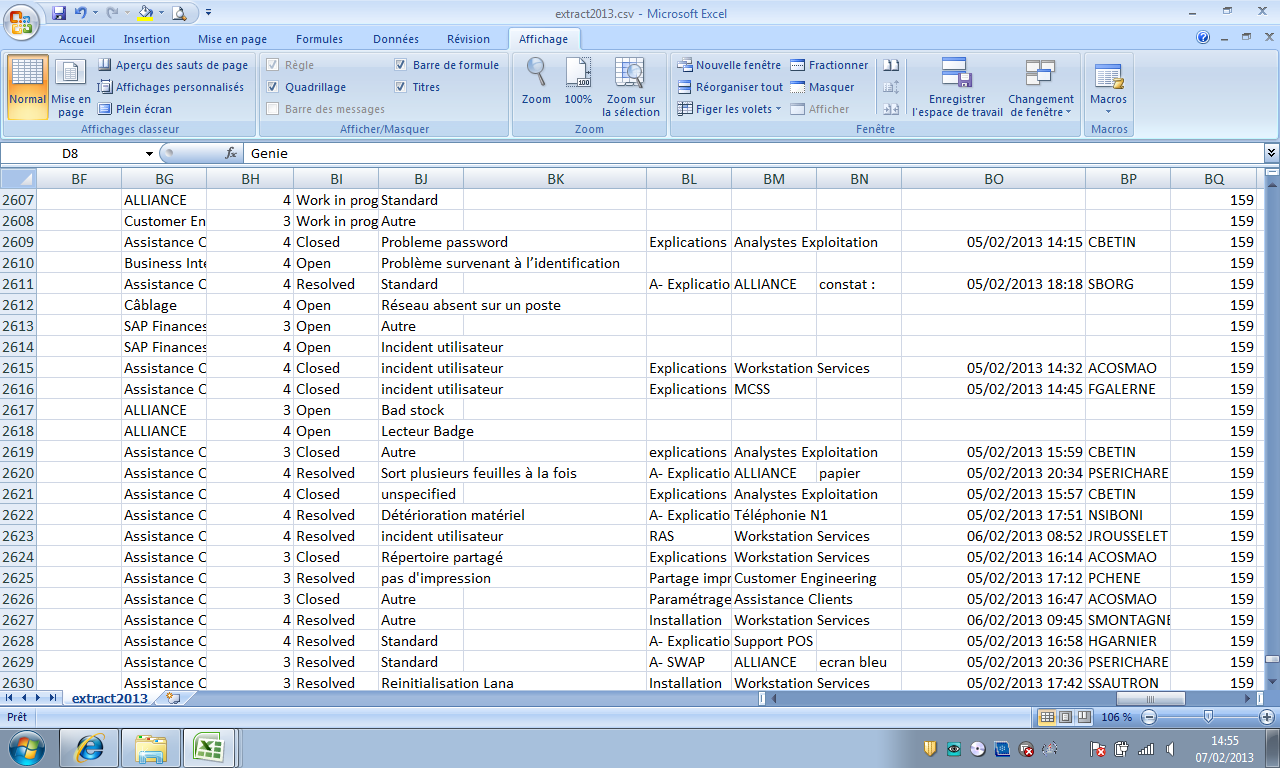
\includegraphics [width=1\textwidth]{images/ExtractSM7.png}
  \end{figure}
\end{center}

J'ai donc effectué un premier tri sur ces données en créant une nouvelle feuille Excel et en y copiant seulement les lignes voulues et les colonnes utilisées. Ce qui donne la figure~\ref{premierTrie} page~\pageref{premierTrie}.
\begin{center}
  \begin{figure}[ht]
    \caption{\label{premierTrie} Extrait de données SM7 après un premier trie}
    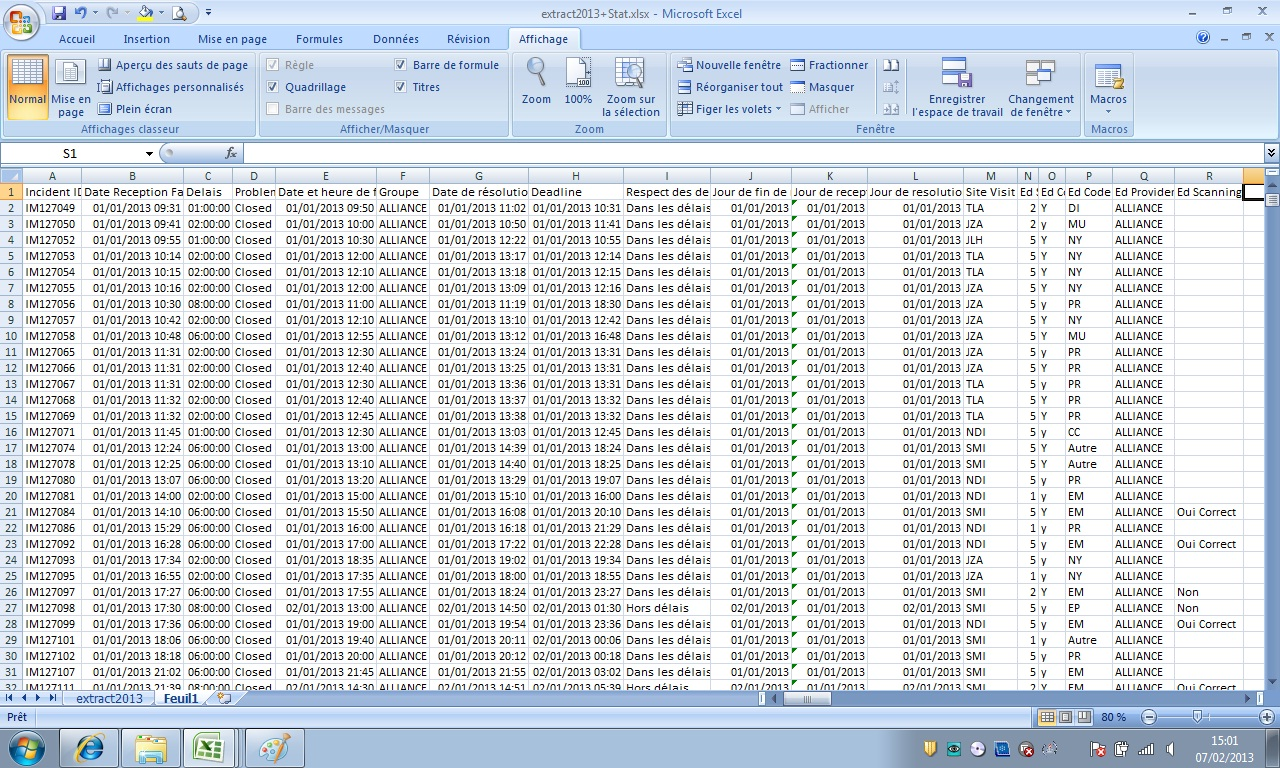
\includegraphics [width=1\textwidth]{images/premierTrie.jpg}
  \end{figure}
\end{center}
C'est donc sur cette feuille que vont se baser la plupart des macros que j'ai réalisé.

\paragraph{}
Une fois ce traitement effectué, j'ai utilisé ces données pour calculer des statistiques. J'ai commencé par créer la macro de "contrôle" mentionnée plus haut. J'ai utilisé des tableaux croisés dynamique et d'autres outils disponibles dans Excel pour arriver facilement à un résultat. 
Les tableaux et statistiques que je calcule sont stockés dans la même feuille que les données. Parmi les statistiques que je calcule, certaines seront copiées directement dans le fichier de productivité des techniciens. 

Le résultat de la macro de "contrôle" correspond aux images~\ref{premierCalculs} page~\pageref{premierCalculs}, \ref{deuxiemeTraitement} page~\pageref{deuxiemeTraitement} et \ref{troisiemeTraitement} page~\pageref{troisiemeTraitement}.
\begin{center}
  \begin{figure}[ht]
    \caption{\label{premierCalculs} Première partie du résultat de la macro "contrôle"}
    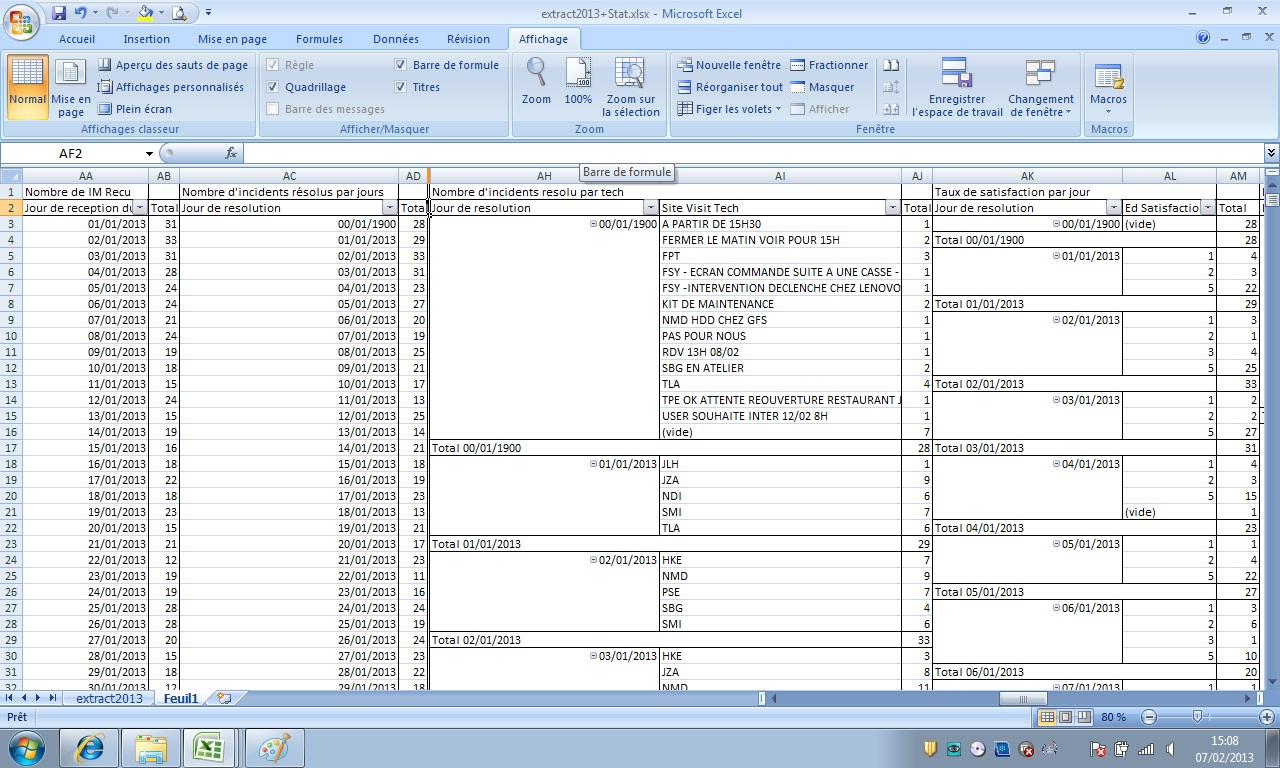
\includegraphics [width=1\textwidth]{images/premierCalculs.jpg}
  \end{figure}
\end{center}
\begin{center}
  \begin{figure}[ht]
    \caption{\label{deuxiemeTraitement} Deuxième partie du résultat de la macro "contrôle"}
    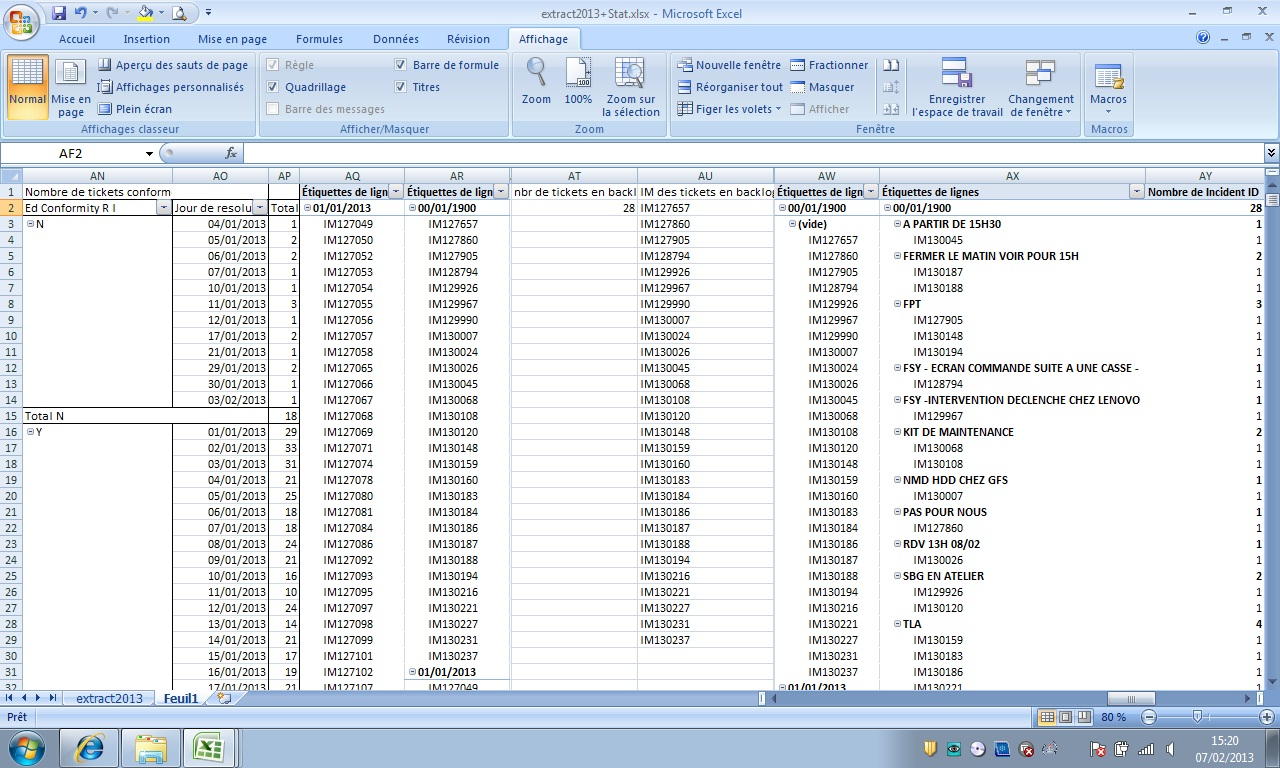
\includegraphics [width=1\textwidth]{images/deuxiemeTraitement.jpg}
  \end{figure}
\end{center}
\begin{center}
  \begin{figure}[ht]
    \caption{\label{troisiemeTraitement} Troisième partie du résultat de la macro "contrôle"}
    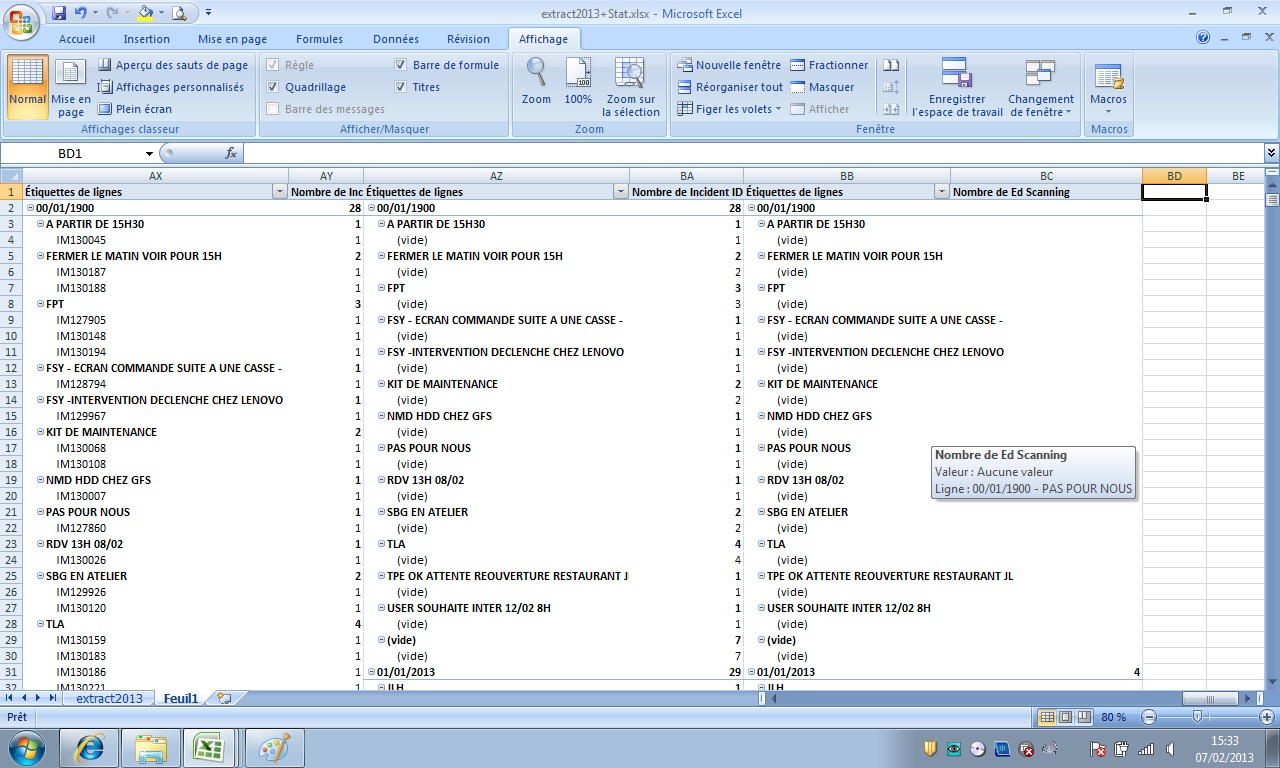
\includegraphics [width=1\textwidth]{images/troisiemeTraitement.jpg}
  \end{figure}
\end{center}

\paragraph{}
%prod des tech 
La macro suivante dont je vais vous parler est celle qui remplit le tableau de bord des techniciens.
Cette macro va ouvrir le fichier à éditer, faire une recherche dedans afin de trouver la feuille, la ligne et la colonne correspondant respectivement au mois, au technicien et au jour à éditer. Enfin la macro copie la valeur depuis le résultat de la première macro dans la case trouvée.

%tab de bord
La troisième macro doit elle aussi modifier un fichier. C'est à peu près le même principe que la macro précédente mais avec une contrainte supplémentaire : certains champs ne devaient pas être écrasés. 
En effet si le champ \gls{backlog} du fichier "tableau de bord" représenté sur l'image~\ref{tableauBordVide} page~\pageref{tableauBordVide} est écrasé alors le \gls{backlog} serait vide (puisque les interventions sont résolues depuis). Sur l'image l'image~\ref{tableauBordVide} page~\pageref{tableauBordVide} on voit donc le tableau de bord vide et sur l'image l'image~\ref{TabBordRempli} page~\pageref{TabBordRempli} on le voit une fois rempli par la macro.
Rappelons que toutes ces opérations étaient effectuées manuellement avant d'être automatisées.
\begin{center}
  \begin{figure}[ht]
    \caption{\label{tableauBordVide} Tableau de bord vide"}
    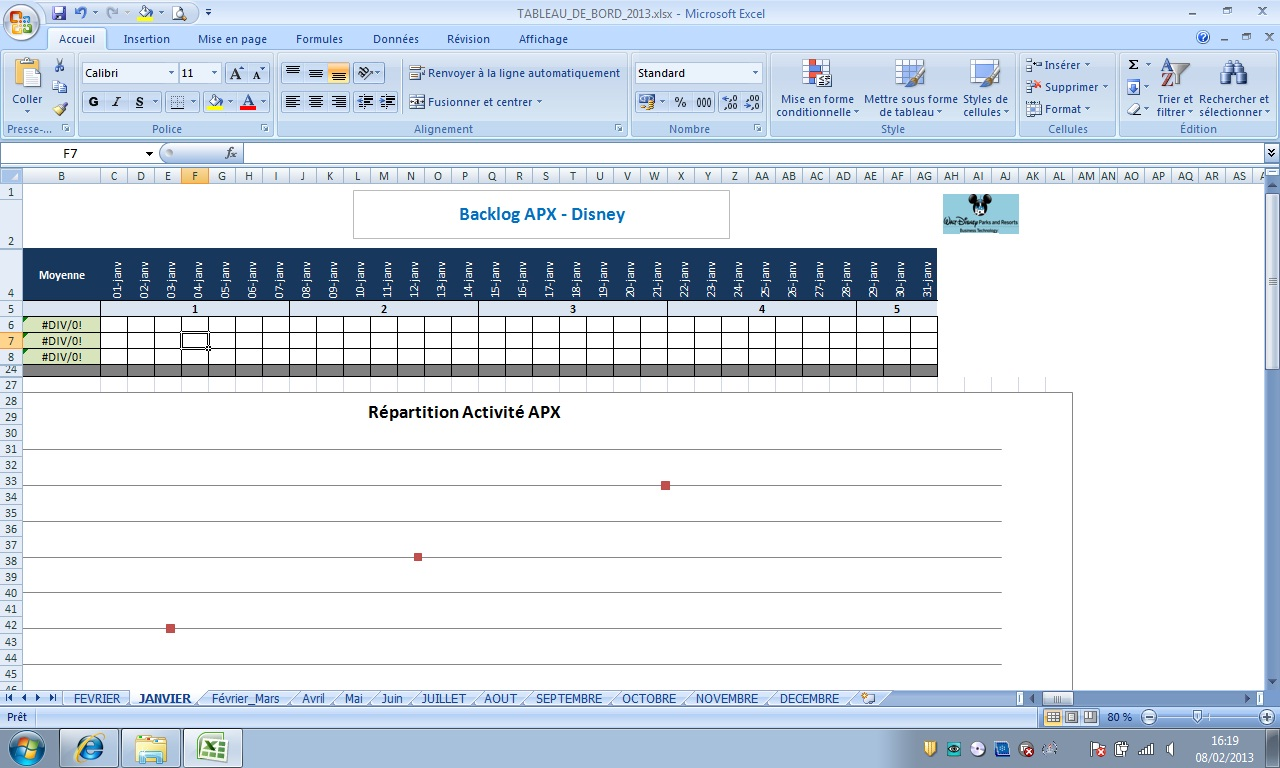
\includegraphics [width=1\textwidth]{images/tableauBordVide.jpg}
  \end{figure}
\end{center}
\begin{center}
  \begin{figure}[ht]
    \caption{\label{TabBordRempli} Tableau de bord après modifications de la macro"}
    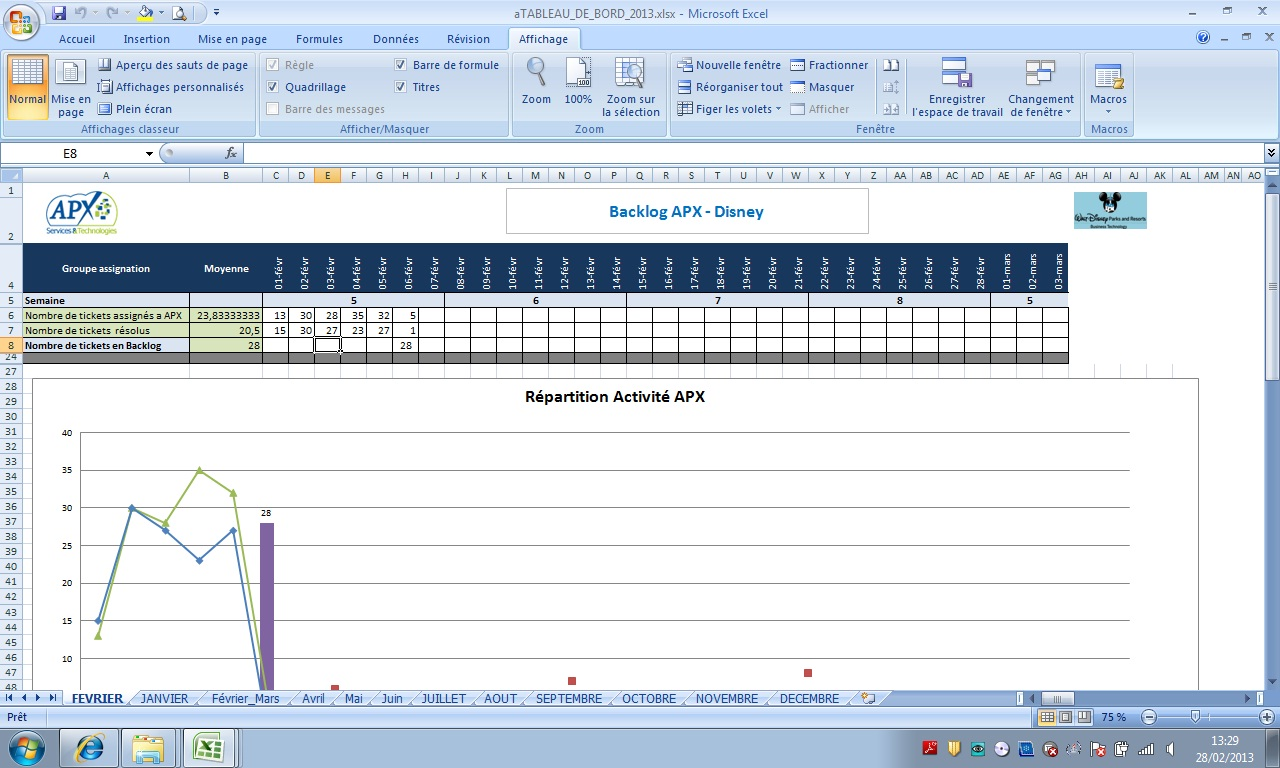
\includegraphics [width=1\textwidth]{images/TabBordRempli.jpg}
  \end{figure}
\end{center}

%listes
Enfin, mes dernières macros ont été plus simple à réaliser, il s'agissait le lister les interventions résolues et en \gls{backlog} avec quelques détails sur l'intervention (cf. figure~\ref{listeResolu} page~\pageref{listeResolu} et figure~\ref{listeBacklog} page~\pageref{listeBacklog}).



\subsection{La mise en production}%
\paragraph{}
Enfin, je voulais vous parler de la mise en production qui à été révélatrice de nombreux problèmes sur les statistiques avant la création de ces macros.
En effet, avant l'automatisation de ces tâches, les données utilisées étaient souvent les \gls{ri} papiers. Or dans certains cas, les \gls{ot} de ces \gls{ri} ont été transférés à un autre service ou bien annulés, mais ils comptais quand même dans nos statistique. Nos statistiques étaient donc faussées.
Avec la création de ces macros, les \gls{ot} annulés ou transférés ne sont pas comptés dans nos statistiques. De plus la feuille issue de la macro de "contrôle" permet de s'en assurer.
J'ai également créé une documentation afin que toutes les étapes nécessaires au bon fonctionnement des macros ne soient pas oubliés. En effet certaines options doivent être cochés dans Excel sans quoi les macros ne peuvent pas êtres lancées par exemple.

\paragraph{}
\newglossaryentry{launcher}{name={\foreignlanguage{english}{launcher}},description={Lanceur}}
Finalement, après de nombreux essais la mise en production de ces macros à été facilitée grâce à une dernière macro. Une macro qui fait office de "\foreignlanguage{english}{\gls{launcher}}\footnote{Lanceur}" de macros. 
J'ai donc crée une petite boite de dialogue où l'utilisateur peut saisir le nom des fichiers à modifier (le tableau de bord, le tableau de productivité des techniciens, etc...) et enfin lancer les macros les unes à la suite des autres (cf. figure~\ref{Launcher} page~\pageref{Launcher} et figure~\ref{nomDesFichiersAEditer} page~\pageref{nomDesFichiersAEditer}).
\begin{center}
  \begin{figure}[ht]
    \caption{\label{Launcher} Launcher de macros"}
    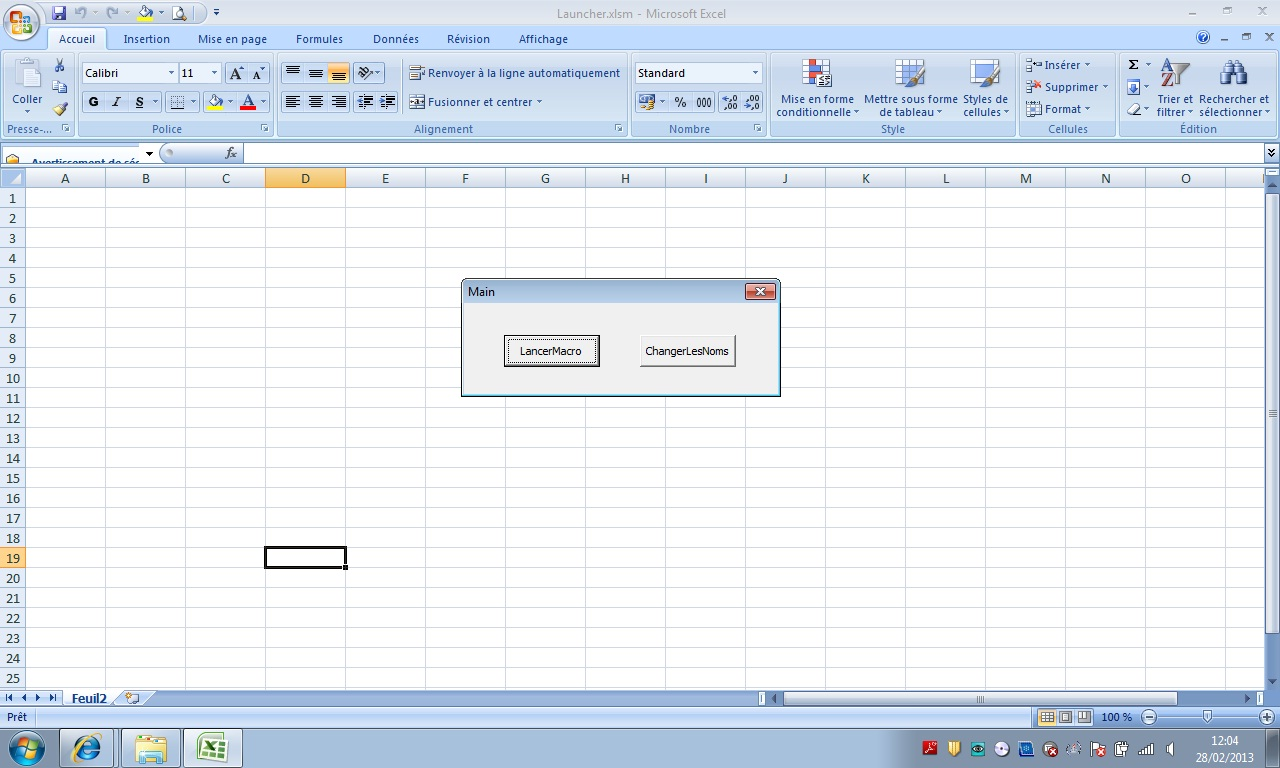
\includegraphics [width=1\textwidth]{images/Launcher.jpg}
  \end{figure}
\end{center}
\begin{center}
  \begin{figure}[ht]
    \caption{\label{nomDesFichiersAEditer} Changement des noms de fichiers dans le launcher"}
    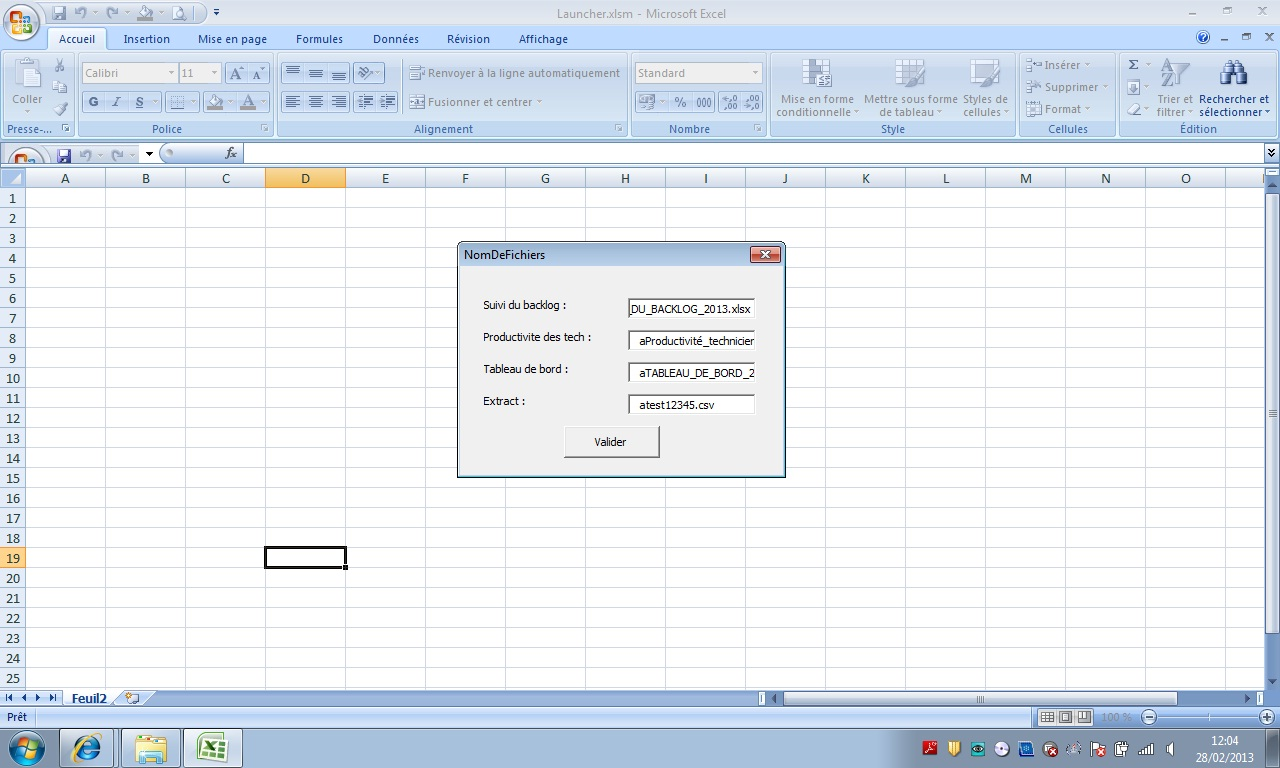
\includegraphics [width=1\textwidth]{images/nomDesFichiersAEditer.jpg}
  \end{figure}
\end{center}

  \cleardoublepage
  % \chapter{Outils d'aide à la planification}
\section{Outils d'aide à la planification}

\subsection{Le contexte}%
\paragraph{}
La gestion de l'emploi du temps d'une équipe de 15 personnes ayant des rythmes différents peut être très problématique. C'est pourquoi, j'ai du réaliser un outils d'aide à la planification. Le but étant d'automatiser un maximum de tâches. 

On peut considérer deux rythmes différents minimum : le rythme des techniciens et le rythme des autres. Le rythme d'un technicien peut changer suivant la semaine et la période. En effet, un technicien peut travailler entre 8 et 10 heures par jour, mais il n'est pas forcé que tous les techniciens travail 7 heures ou 10 heures. Un roulement entre les techniciens peut se faire. 
Dans la suite du rapport on appellera une "plage horaire" un "rythme" correspondant à un ou plusieurs techniciens.
On considère aussi qu'une journée est composée de plusieurs plages horaires et qu'une semaine compte sept jours ouvrables de 8 heures à 23 heures.

\paragraph{}
On définit comme contrainte une limite que l’outil doit pendre en compte lorsqu'il génère un emploi du temps. Par exemple : un technicien doit avoir un weekend de deux jours consécutifs minimum par semaine. 
La première liste de contraintes à respecter est celle du Code du Travail. Cependant, au delà du code du travail, d'autres contraintes sont définies. Parmi elles ont peut cité par exemple : 
\begin{enumerate}
  \item Au moins 5 techniciens doivent être présent par jour
  \item Il ne doit pas y avoir de trous dans la journée d'un technicien
  \item 2 techniciens doivent commencer leur journée à 8 heures et 2 techniciens doivent terminer à 23 heures
\end{enumerate}
La gestion de l'emploi du temps est très problématique car les jours fériés et les dimanches sont travaillés et donc majorés. De plus certains techniciens ont des enfants à charge, ils ne peuvent donc pas avoir des horaires aussi flexibles que les autres.




\subsection{La réalisation}%
\paragraph{}
\newacronym{api}{API}{\foreignlanguage{english}{Application Programming Interface (Interface de programmation)}}
\newglossaryentry{apidef}{name={interface de programmation},description={Une interface de programmation est une façade clairement délimitée par laquelle un logiciel offre des services à d'autres logiciels. cf. \url{http://fr.wikipedia.org/wiki/Interface_de_programmation}}}

\newacronym{dom}{DOM}{\foreignlanguage{english}{Document Object Model}}
\newglossaryentry{domdef}{name={Document Object Model},description={Standard indépendant de tout langage de programmation permettant la modification de documents XML et HTML. cf. \url{http://fr.wikipedia.org/wiki/Document_Object_Model}}}
Afin de répondre au mieux aux attentes de l'équipe de techniciens et au maître d'apprentissage, j'ai demandé l'avis de quelques professeurs quant à la réalisation technique de cette outil. M.~Chan \textsc{Leduc} m'a suggéré un projet de fin d'année collant parfaitement avec ma mission en entreprise. Parmis les solutions techniques retenues, il y a Alloy(cf. figure~\ref{GUIalloy} page~\pageref{GUIalloy}), un langage déclaratif qui permet de mettre en place simplement un modèle représentatif d'un emploi du temps. 
Afin d'illustrer mon propos, l'image~\ref{solution} page~\pageref{solution} représente la solution (avant d'être interpréter) issue du modèle Alloy de mon entreprise.
\begin{center}
  \begin{figure}[ht]
    \caption{\label{GUIalloy} Interface graphique d'Alloy}
    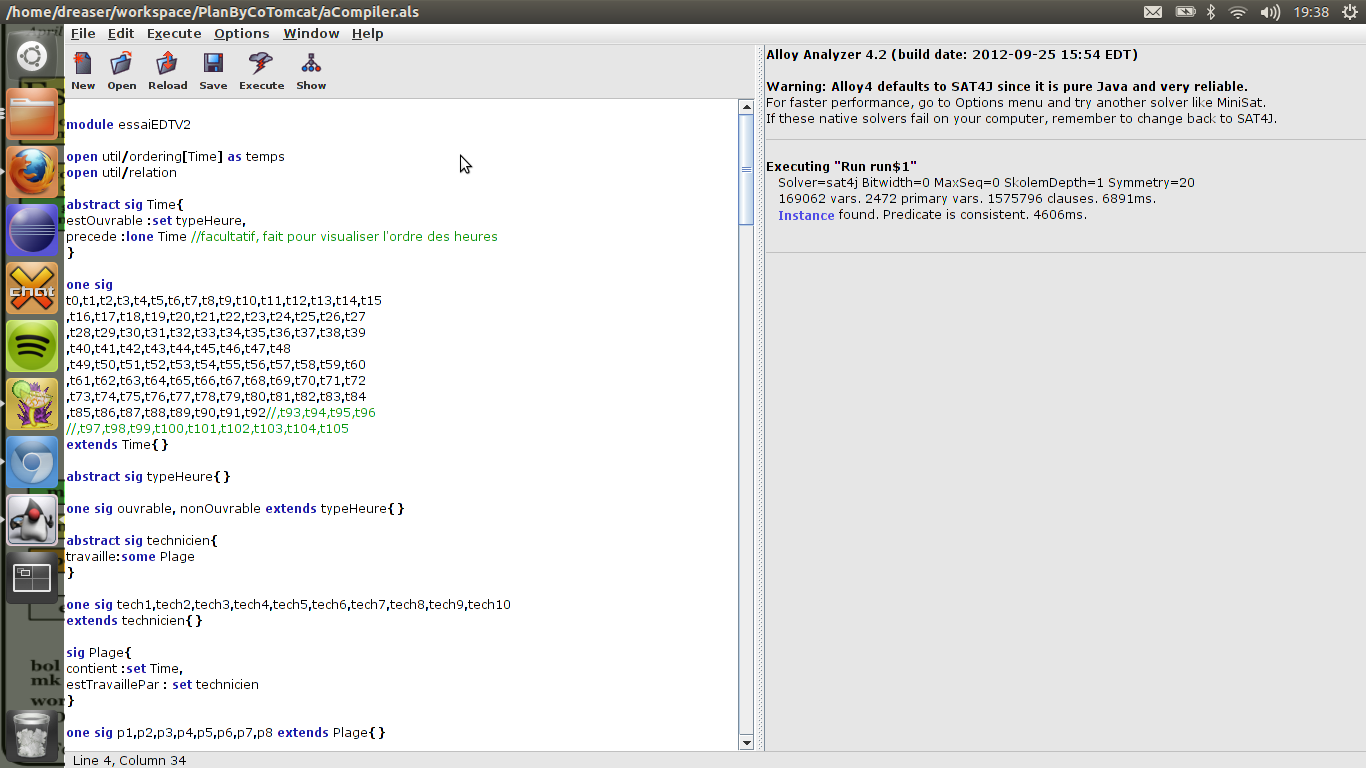
\includegraphics [width=1\textwidth]{images/alloy/GUIalloy.png}
  \end{figure}
\end{center}
\begin{center}
  \begin{figure}[hb]
    \caption{\label{solution} Solution issue du modèle Alloy de mon entreprise}
    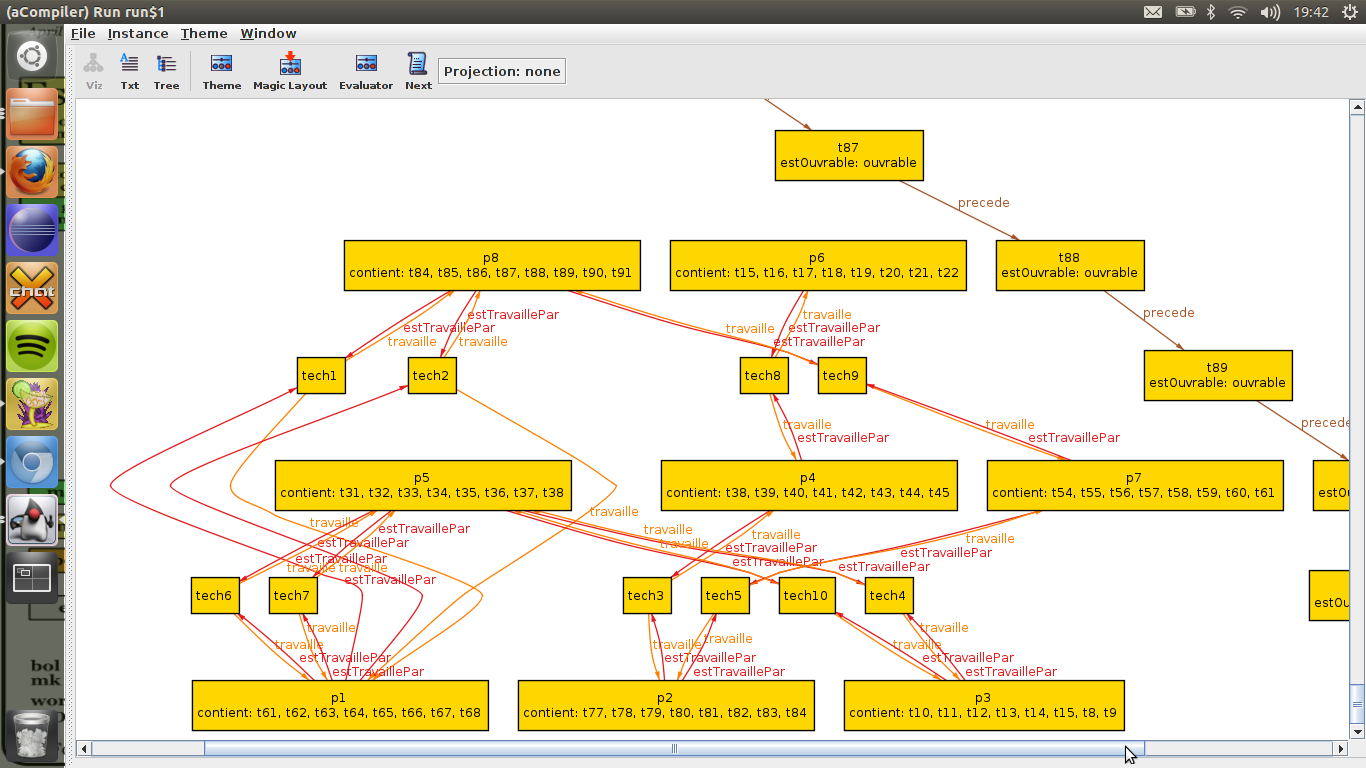
\includegraphics [width=1\textwidth]{images/alloy/solution4j10t.png}
  \end{figure}
\end{center}

La difficulté majeur reposait sur la manière d'exprimer les contraintes. Une contrainte est exprimée de la manière suivante : 
\begin{Verbatim}[frame=single,numbers=left]
//Toutes les plages doivent etre travaillees par au moin un tech
fact{
all p : Plage | some tec : technicien | tec->p in travaille
}
\end{Verbatim}

L'élaboration du modèle Alloy a été la phase la plus difficile de cette mission. Elle a mobilisée une grande partie des mes connaissances mathématiques. C'est finalement avec l'aide de M.\textsc{Bonnot} que j'ai réussi à établir un modèle répondant aux exigences.
Nous avons également choisi de mettre en place un serveur web open-source codé en Java afin de pouvoir le modifier à notre guise. Le fait que le serveur soit codé en Java nous permet également de "piloter" l'\gls{api}\footnote{Une \gls{apidef} est une façade clairement délimitée par laquelle un logiciel offre des services à d'autres logiciels. cf. \url{http://fr.wikipedia.org/wiki/Interface_de_programmation}} via un navigateur internet.
Nous avons d'abord choisi Jetty (une version ancienne car plus facile à modifier), puis j'ai migré vers Tomcat qui s'avère être beaucoup plus flexible et plus simple à manipuler.
Jetty à de nombreux défauts, il ne permettait qu'une réponse en une seul ligne par exemple. De plus chaque requête envoyé par le client devait être gérée manuellement.
\paragraph{}
J'ai également utilisé le \gls{dom}\footnote{Le \gls{domdef} est un standard indépendant de tout langage de programmation permettant la modification de documents XML et HTML. cf. \url{http://fr.wikipedia.org/wiki/Document_Object_Model}} pour générer et interpréter la solution proposée par le compilateur Alloy.
Cette mission n'étant pas achevée, je n'ai pas travaillé l'apparence de l'outil.

\paragraph{}
Parlons maintenant du fonctionnement de l'outil du point de vue du serveur.
Lorsque le serveur reçoit une requête du client, il l'utilise pour recréer le modèle Alloy à partir des différents morceaux stockés dans des fichiers XML. Une fois que le modèle Alloy est reconstitué, il est compilé avec l'\gls{api}. Le résultat est finalement interprété avec le \gls{dom} pour modifier les fichiers HTML qui seront retournés au client.



\subsection{Fonctionnement du point de vue client}%
\paragraph{}
Lorsque l'utilisateur entre l'adresse du site, le serveur renvoi une première page d'accueil avec une première proposition d'emploi du temps "sans contraintes" et un formulaire pour ajouter des contraintes. L'utilisateur peut désormais saisir une première contrainte concernant un technicien en particulier ou une plage horaire en particulier. 
Un nouvelle emploi du temps est généré et retourné au client. Ainsi le client peut modifier à volonté l'emploi du temps.
L'affichage est maintenant beaucoup plus flexible après la migration vers Tomcat étant donnée que Tomcat permet l'utilisation de "Java" dans une page HTML : 
\begin{Verbatim}[frame=single,numbers=left]
<html>
<body>
<table align="center" border="1" summary="" width="80%">
<% 
ArrayList<Jour> attribut = (ArrayList<Jour>)
 request.getAttribute("liste");
for (Jour j : attribut){
	out.println("<tr>");
	out.println("<td>");
	out.println("<b>"+j.getNom()+"</b>");
	out.println("</td>");
	for (PlageHoraire plage : j.getPlagesHoraires()){
		out.println("<td>");
		out.println(plage.getNomPlageHoraire());
		out.println("</td>");
	}
	out.println("</tr>");
}
%>
</table>
</body>
</html>
\end{Verbatim}


Aucune sécurité n'a été mise en place (pour le moment) afin d'éviter que les techniciens ne modifient l'emploi du temps à leur gré sans l'accord du manager.
Toutes les connexions en tant qu'admin ou autres seront gérées en Java directement, donc pas de PHP.
L'archivage des emplois du temps n'est pas non plus opérationnel. Pour l'instant l'emploi du temps est recalculé et stocké à chaque requête  dans un fichier XML. Aucune base de donnée n'est nécessaire.
La seul contrainte inhérente au serveur est qu'il nécessite une machine virtuelle Java.
En effet, du côté client, le site ne nécessite rien d'autre qu'un navigateur supportant le HTML5. 

  \cleardoublepage
  \section*{Conclusion}
\addcontentsline{toc}{section}{Conclusion}

qsfq sqf

  \cleardoublepage
  
%   \chapter*{Références}
\addcontentsline{toc}{chapter}{Références}


  \nocite{*}
% \begin{multicols}{2}
%   \printglossaries
  \printglossary[type=\acronymtype, title=Acronymes, toctitle=Acronymes]
  \printglossary[toctitle=Glossaire]

% \end{multicols}

%   \begin{resume}
%   xdvxwcvxcvx
%   \end{resume}
%   \begin{abstract} 
%   the same in english 
%   \end{abstract}
  \bibliographystyle{plain-fr}
  \bibliography{biblio}
  
  \appendix
  
\addtocontents{toc}{\newpage \vskip 10 mm \Large \centerline {\textsc{Annexes}} \normalsize \vskip 5mm}
\part*{\Huge{Annexes}}
% \setcounter{page}{1} % Réinitialisation du compteur
% \pagenumbering{arabic}

  \chapter*{Création du launcher}
\addcontentsline{toc}{chapter}{Création du launcher}

\begin{center}
  \begin{figure}[ht]
    \caption{\label{mainLauncher} On fait un appel à une méthode d'une feuille depuis le classeur}
    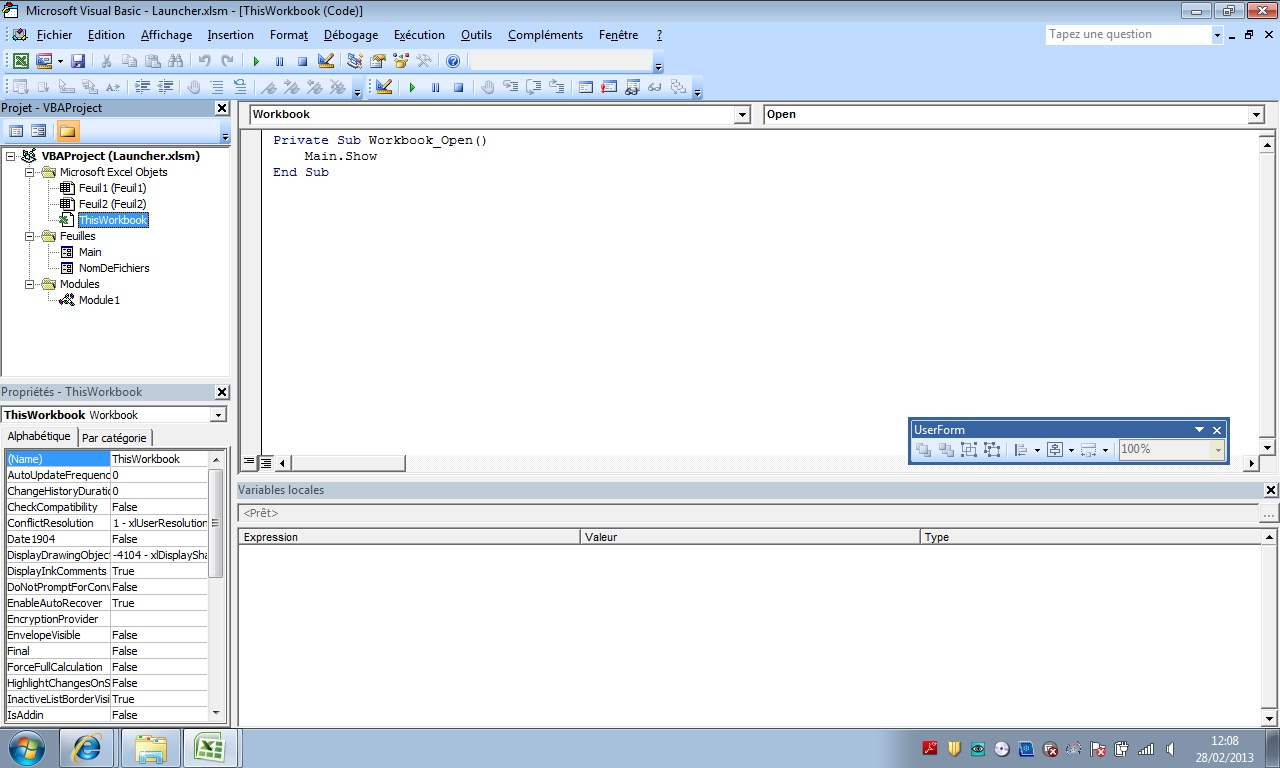
\includegraphics [width=1\textwidth]{images/aMainLauncher.jpg}
  \end{figure}
  \begin{figure}[ht]
    \caption{\label{InterfaceUserFormMain} Création d'u launcher}
    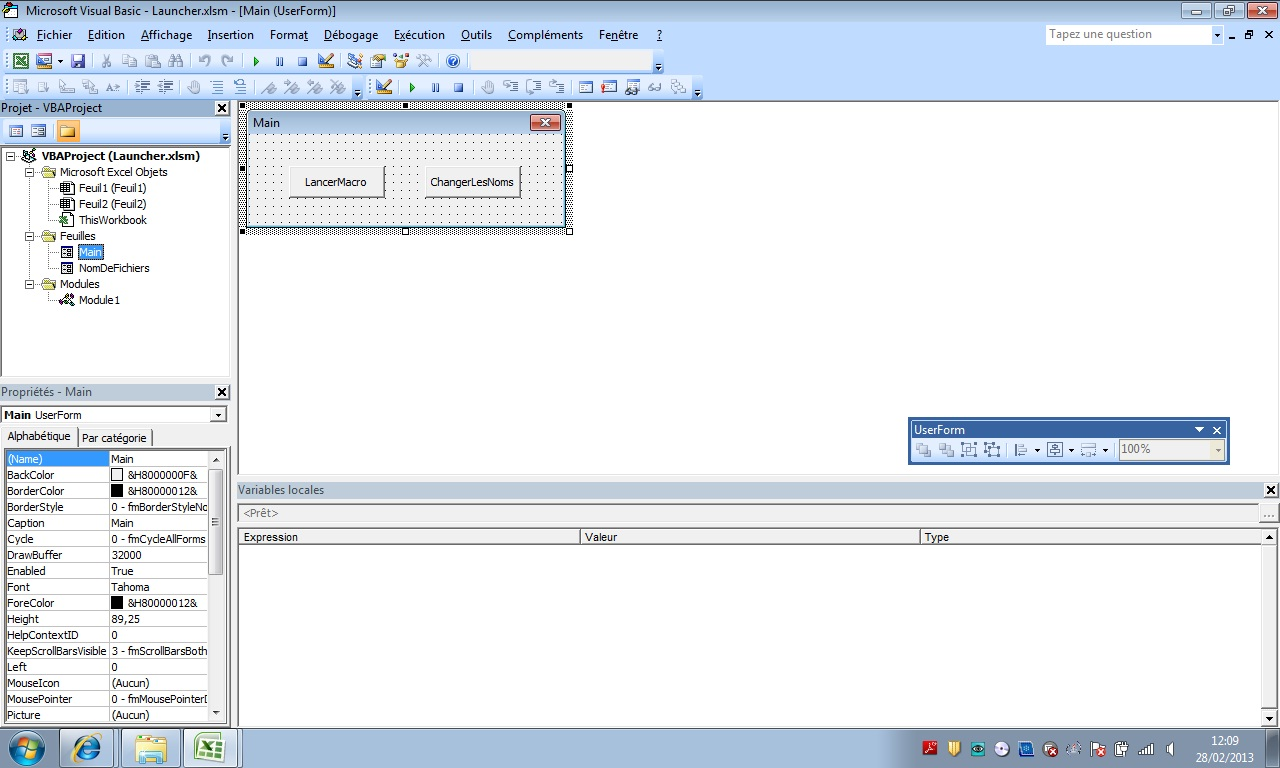
\includegraphics [width=1\textwidth]{images/InterfaceUserFormMain.jpg}
  \end{figure}
  \begin{figure}[ht]
    \caption{\label{InterfaceUserFormNoms} Création d'une boite de dialogue}
    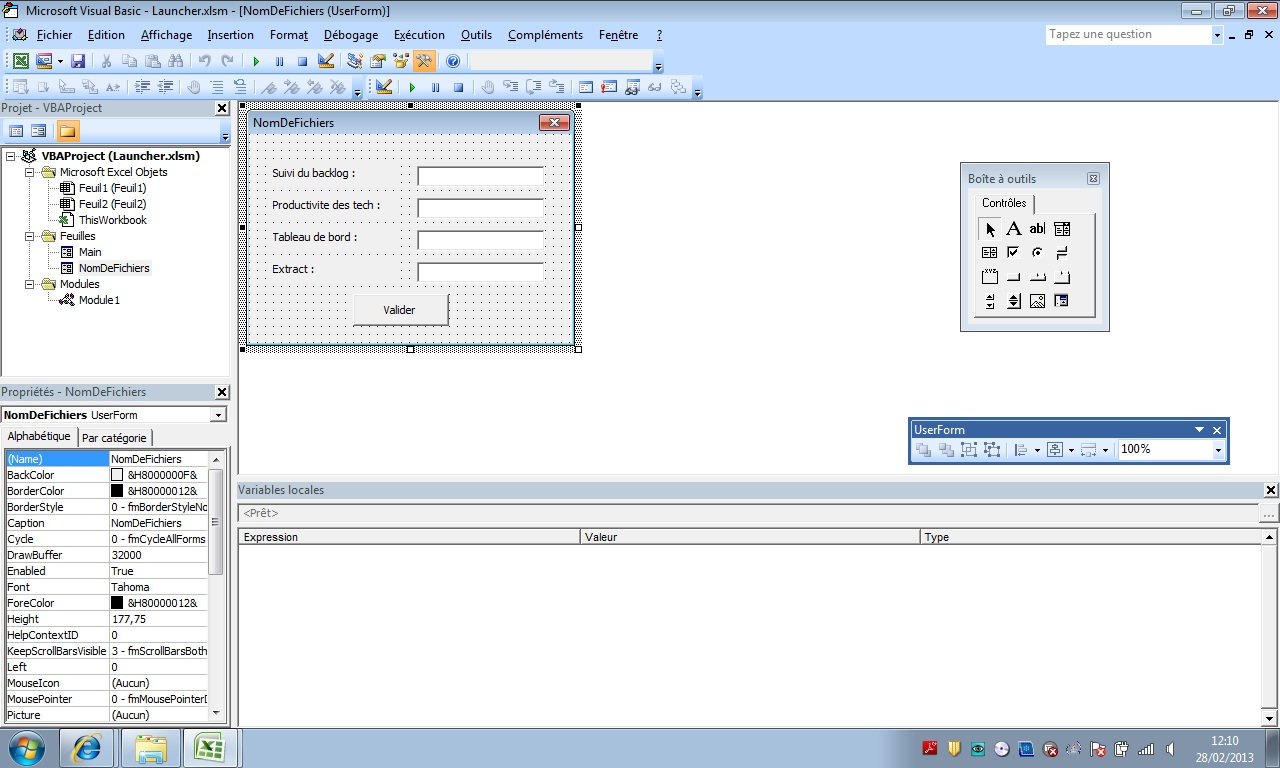
\includegraphics [width=1\textwidth]{images/InterfaceUserFormNoms.jpg}
  \end{figure}
  \begin{figure}[ht]
    \caption{\label{CodeUserFormMain} Méthodes appelés lors d'un clic sur les boutons}
    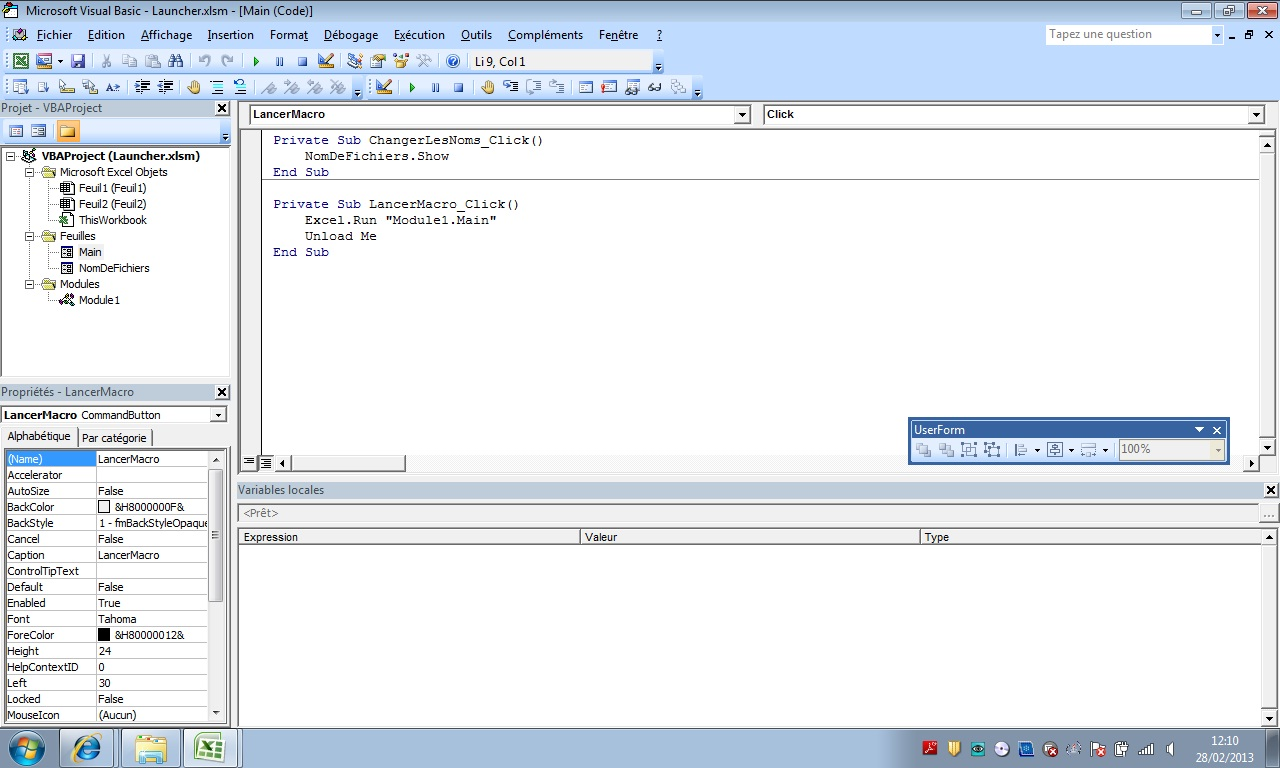
\includegraphics [width=1\textwidth]{images/code/CodeUserFormMain.jpg}
  \end{figure}
  \begin{figure}[ht]
    \caption{\label{CodeMacroLauncher} Code exécuté au clic sur le bouton "lancerMacro"}
    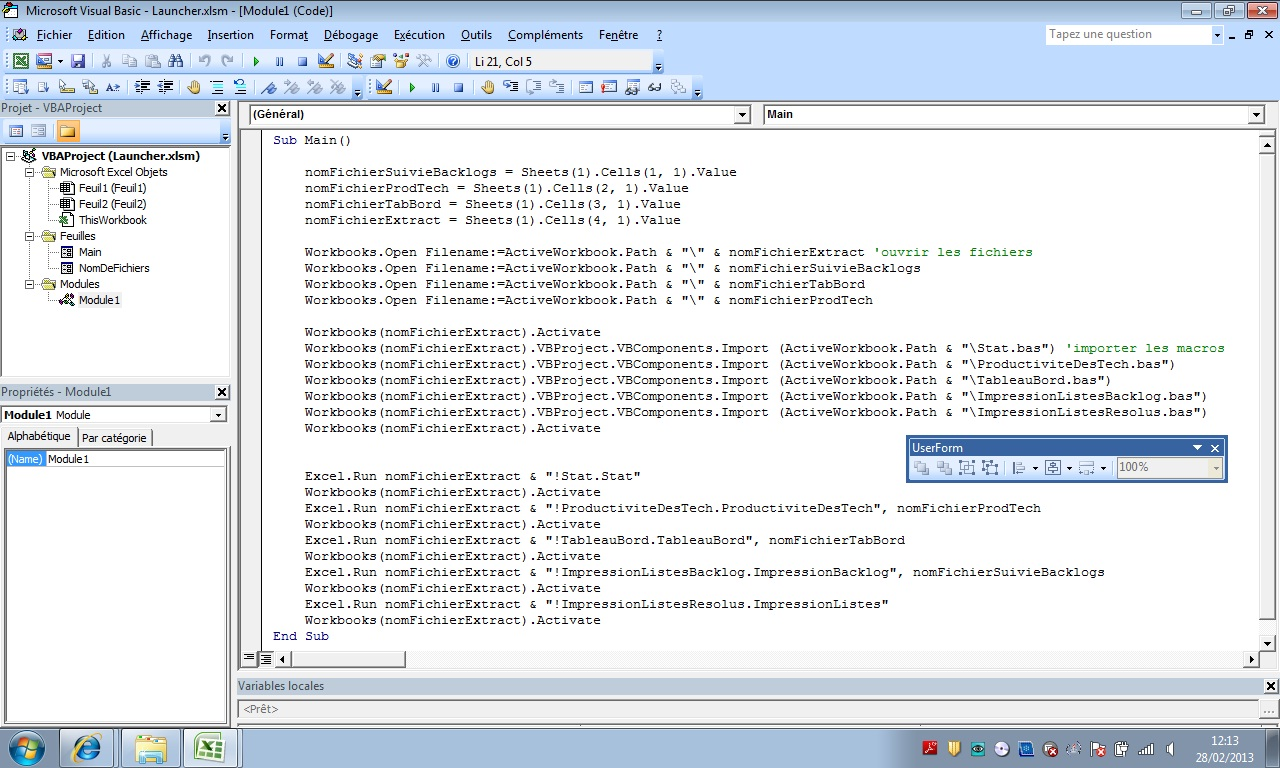
\includegraphics [width=1\textwidth]{images/code/CodeMacroLauncher.jpg}
  \end{figure}
  \begin{figure}[ht]
    \caption{\label{CodeUserFormNoms} Code exécuté au clic sur le bouton "changerLesNoms"}
    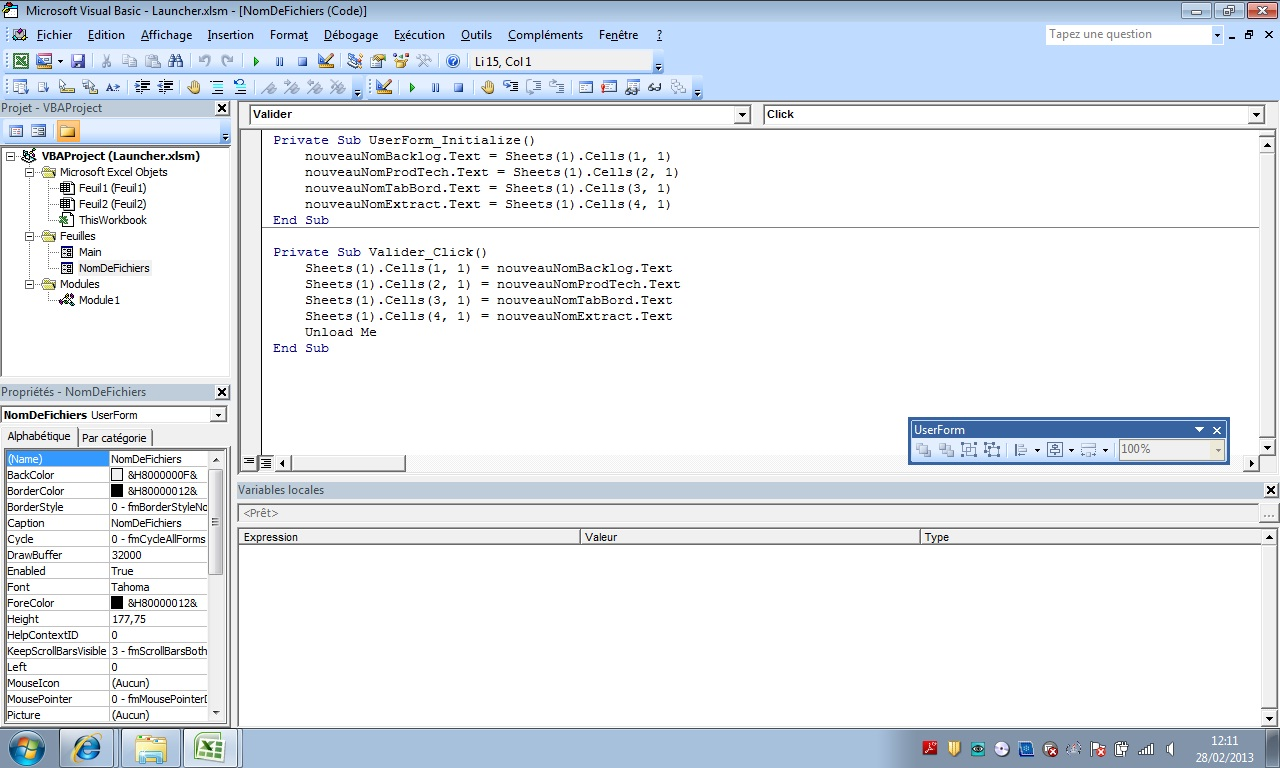
\includegraphics [width=1\textwidth]{images/code/CodeUserFormNoms.jpg}
  \end{figure}
  \begin{figure}[ht]
    \caption{\label{CodeMacroProdTechAnnexe} Code de la macro "productiviteDesTechs"}
    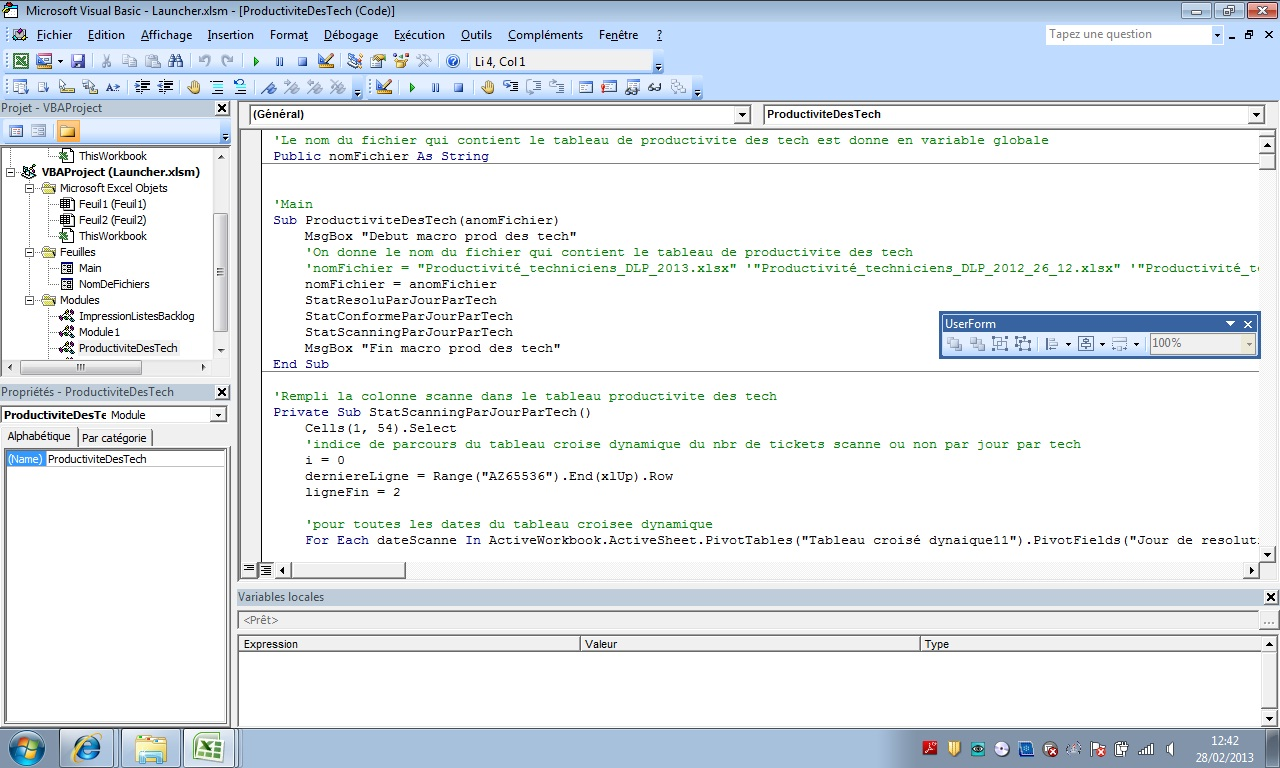
\includegraphics [width=1\textwidth]{images/code/CodeMacroProdTechAnnexe.jpg}
  \end{figure}
\end{center}

\cleardoublepage
\chapter*{Documention}
\addcontentsline{toc}{chapter}{Documention}


\begin{center}
\textbf{HowTo Launcher}
\end{center}
\lstinputlisting{doc/HowTo.txt}

\begin{center}
\textbf{Doc Launcher}
\end{center}
\lstinputlisting{doc/readmeLauncher.txt}

\begin{center}
\textbf{Doc généralee}
\end{center}
\lstinputlisting[breaklines]{doc/readmeMain.txt}

\begin{center}
\textbf{Doc macro contrôle}
\end{center}
\lstinputlisting[breaklines]{doc/readmeStats.txt}

\cleardoublepage
\chapter*{Matériel dépanné et locaux}
\addcontentsline{toc}{chapter}{Matériel dépanné}

\begin{center}
  \begin{figure}[ht]
    \caption{\label{tpe} Quelques appareils réparé (scannette(g), terminal de paiement électronique, imprimante à tickets de caisse(d)"}
    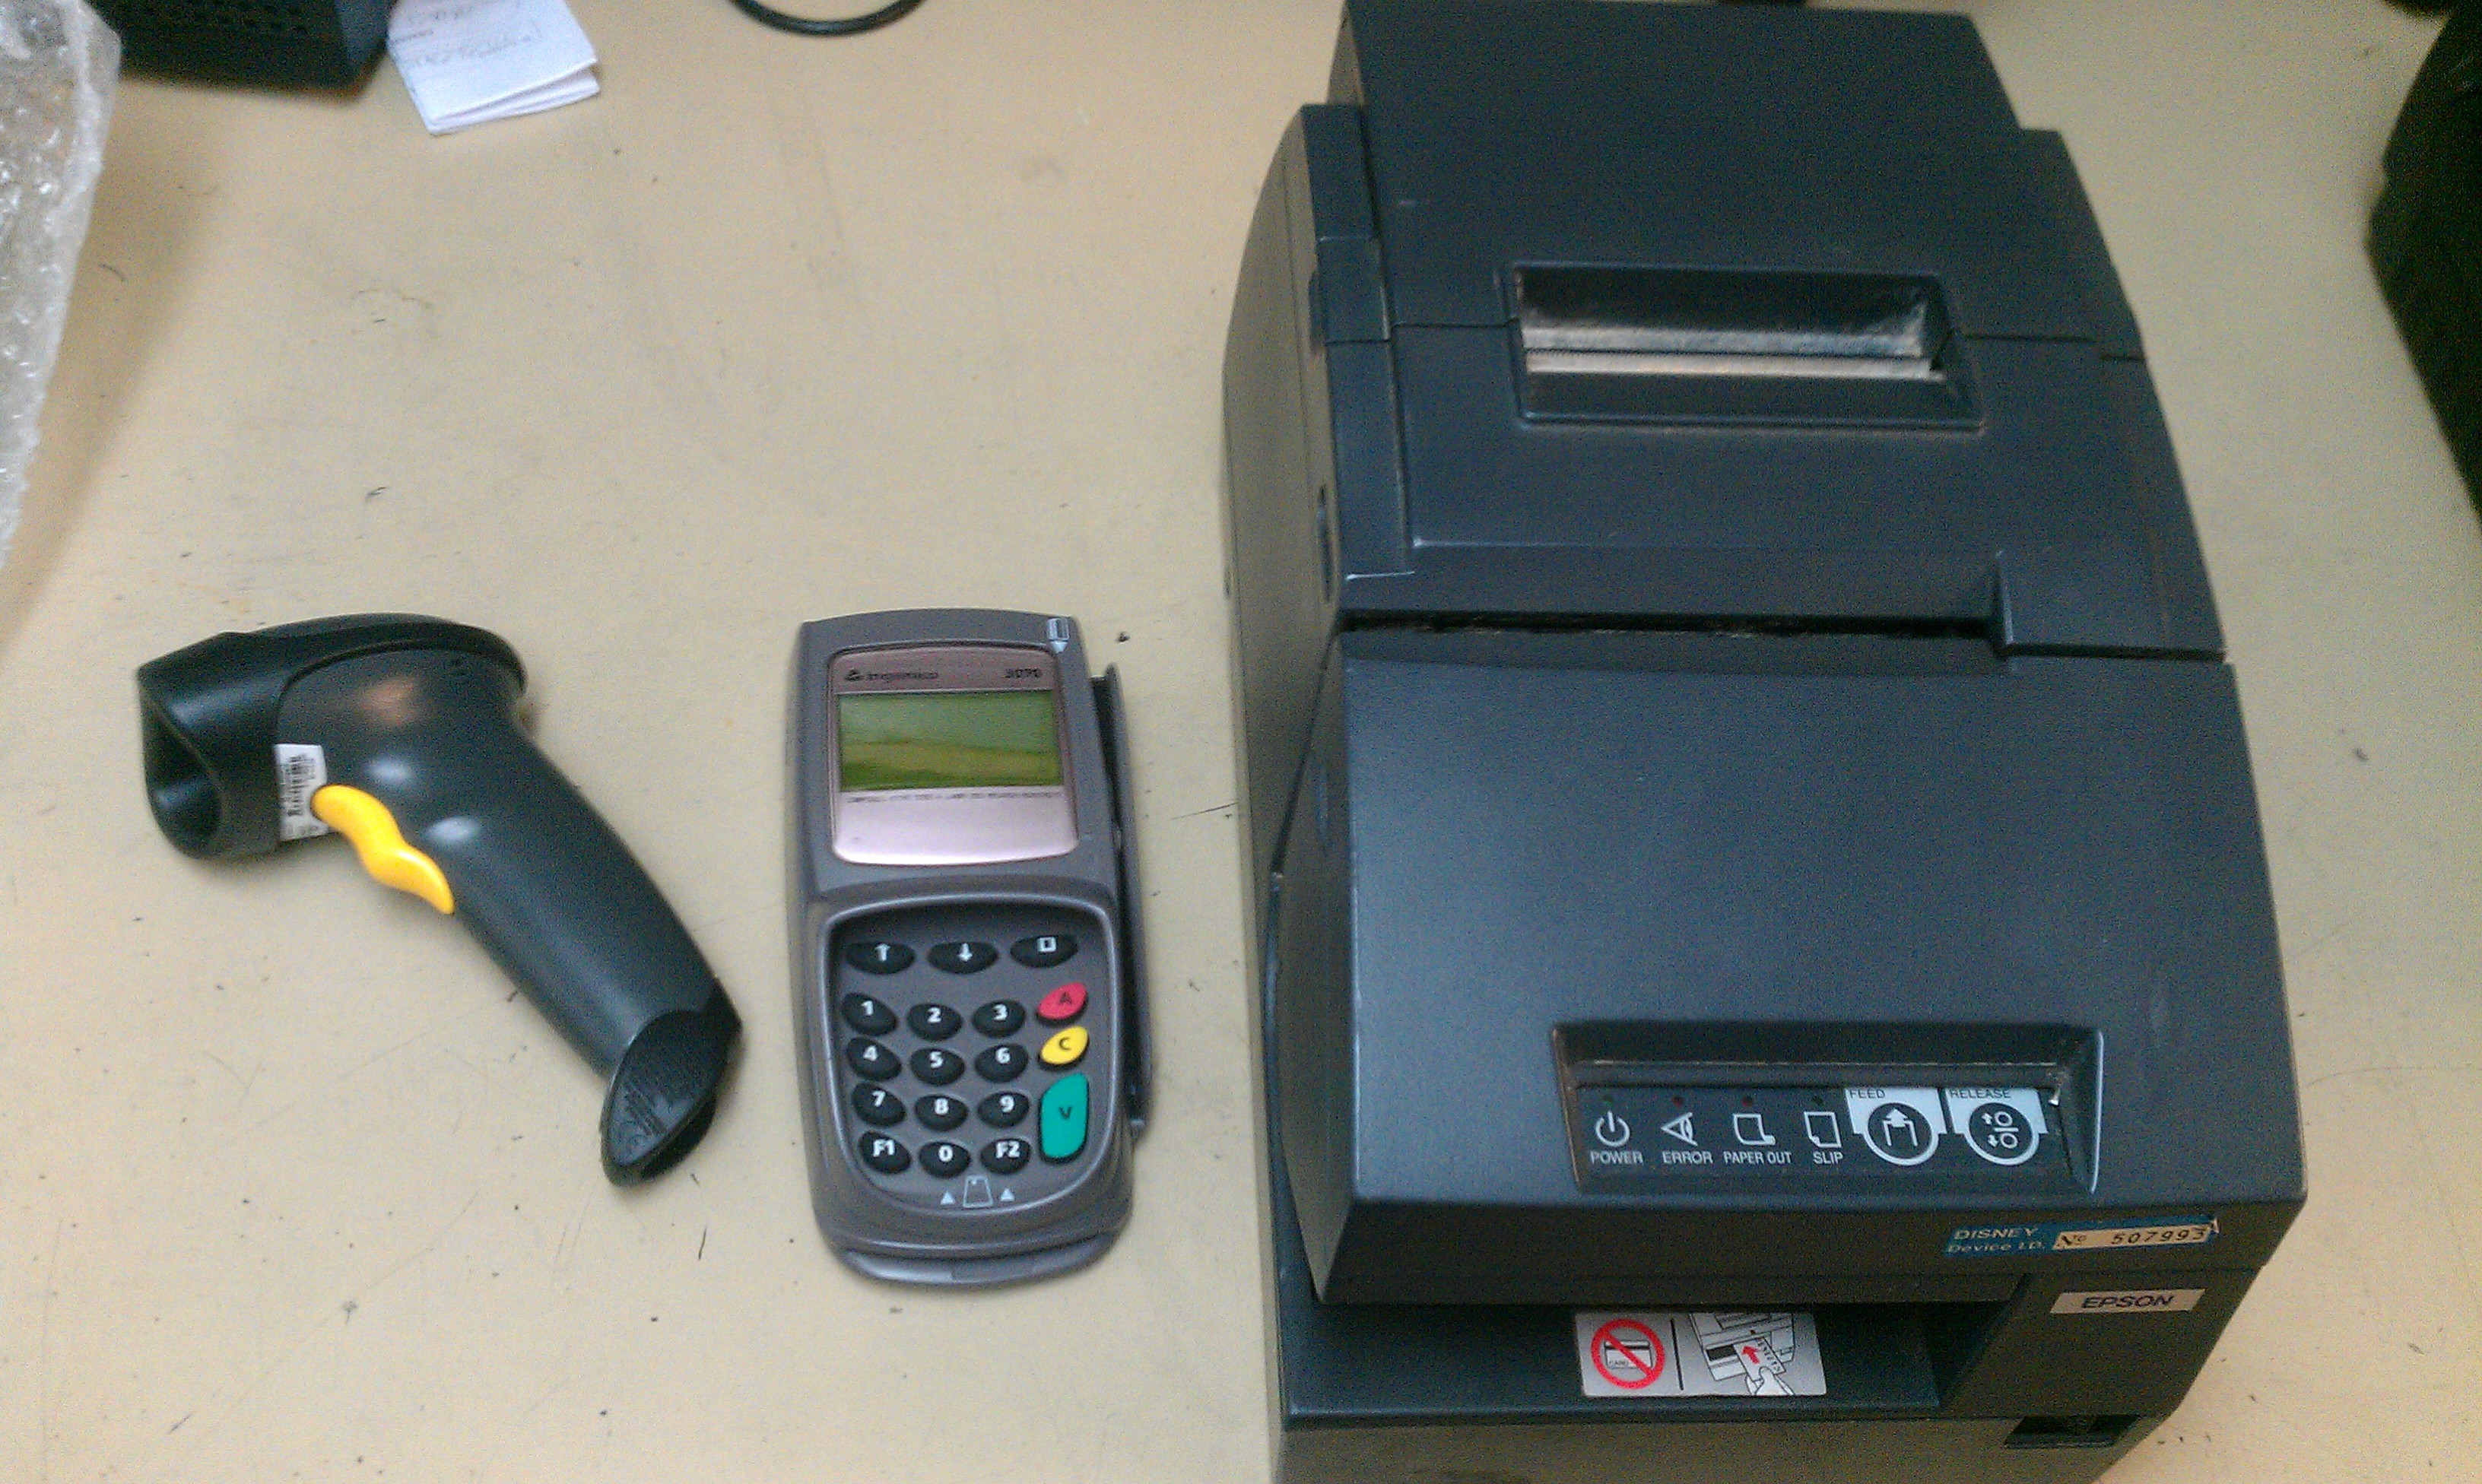
\includegraphics [width=1\textwidth]{images/tpe.jpg}
  \end{figure}
  \begin{figure}[ht]
    \caption{Le stock}
    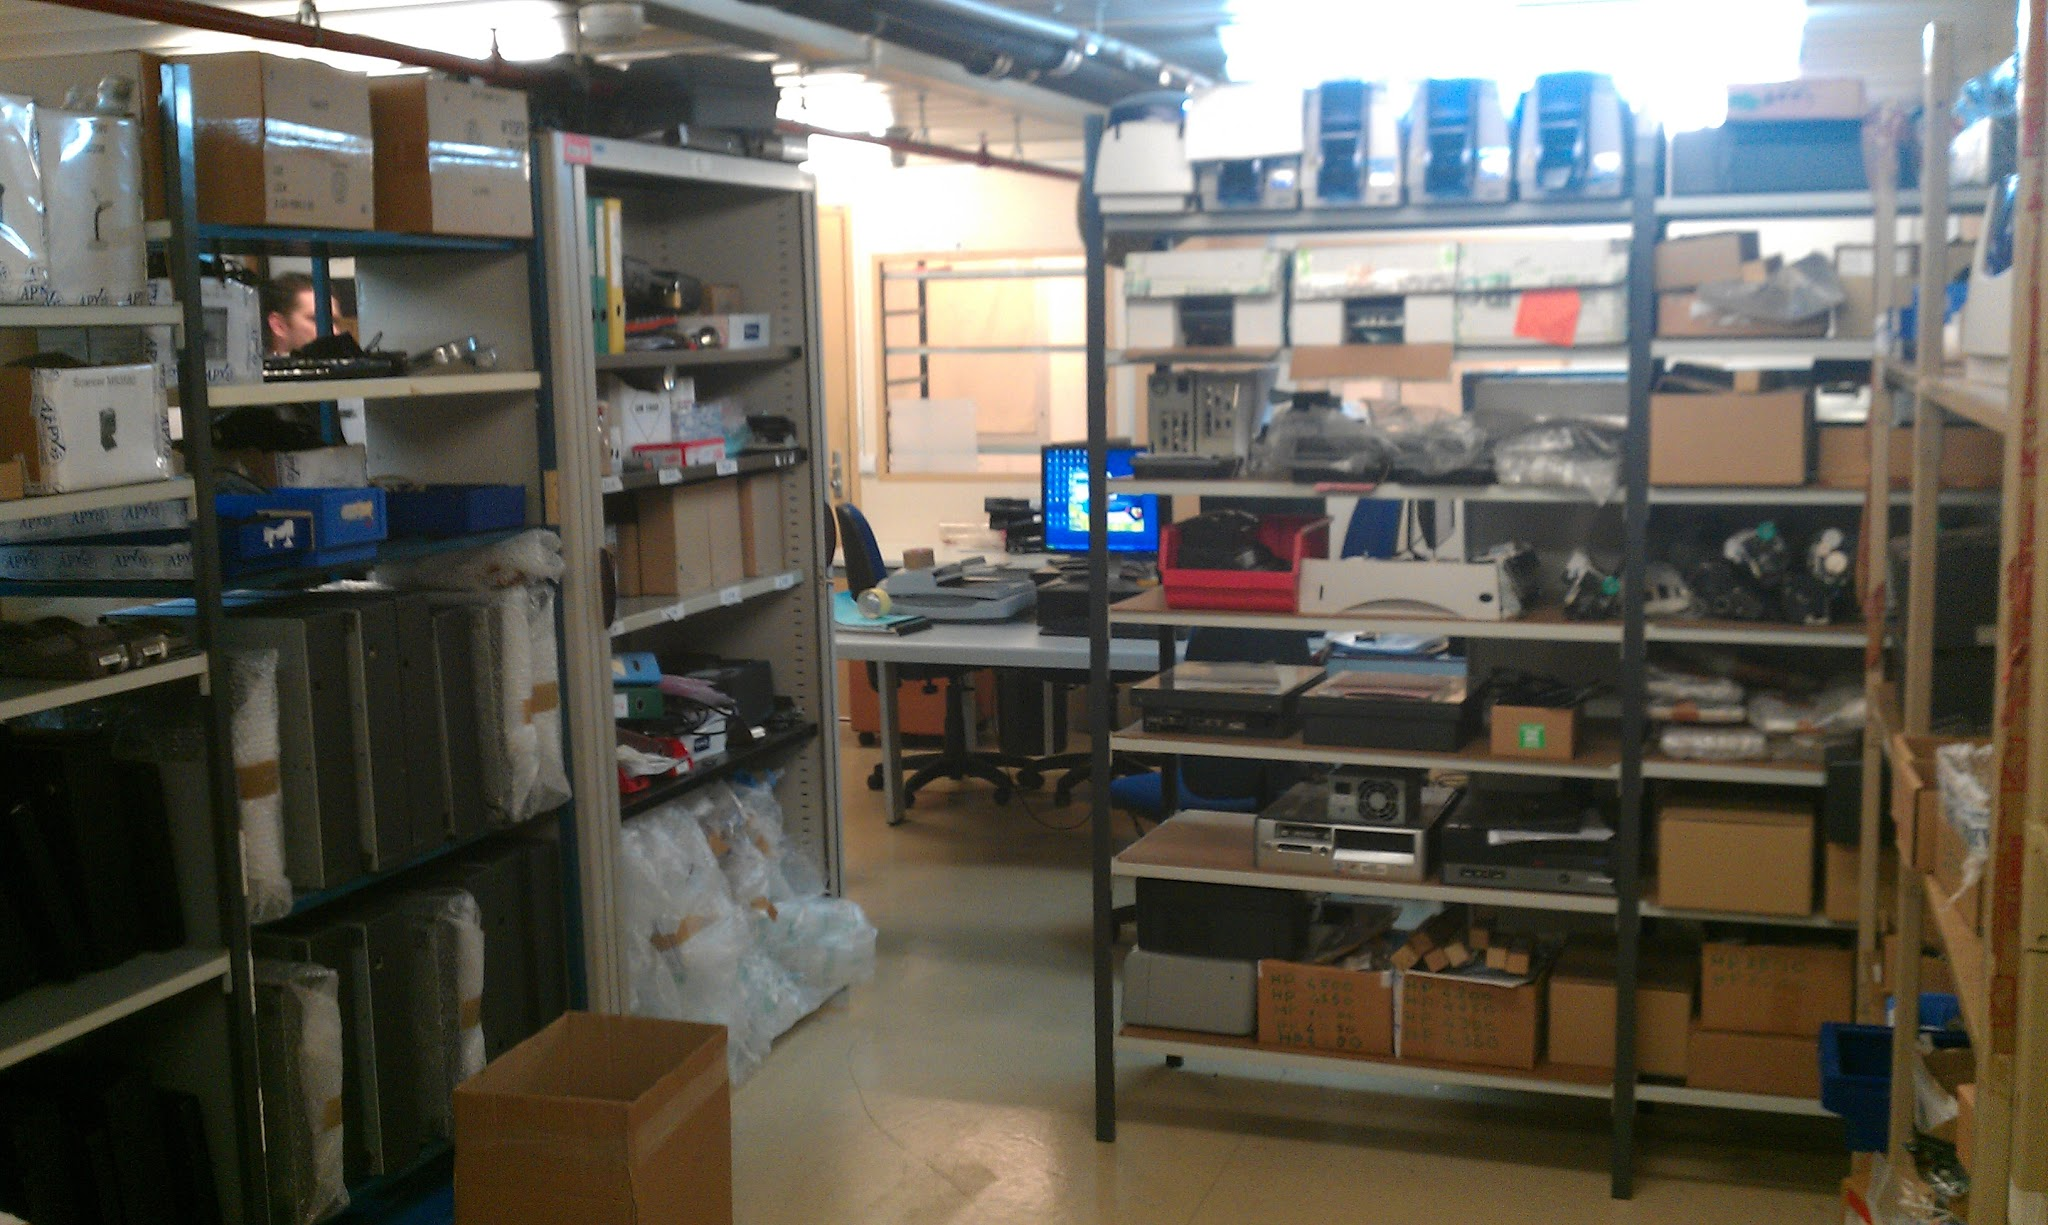
\includegraphics [width=1\textwidth]{images/locaux/IMAG0392.jpg}
  \end{figure}
  \begin{figure}[ht]
    \caption{Le stock}
    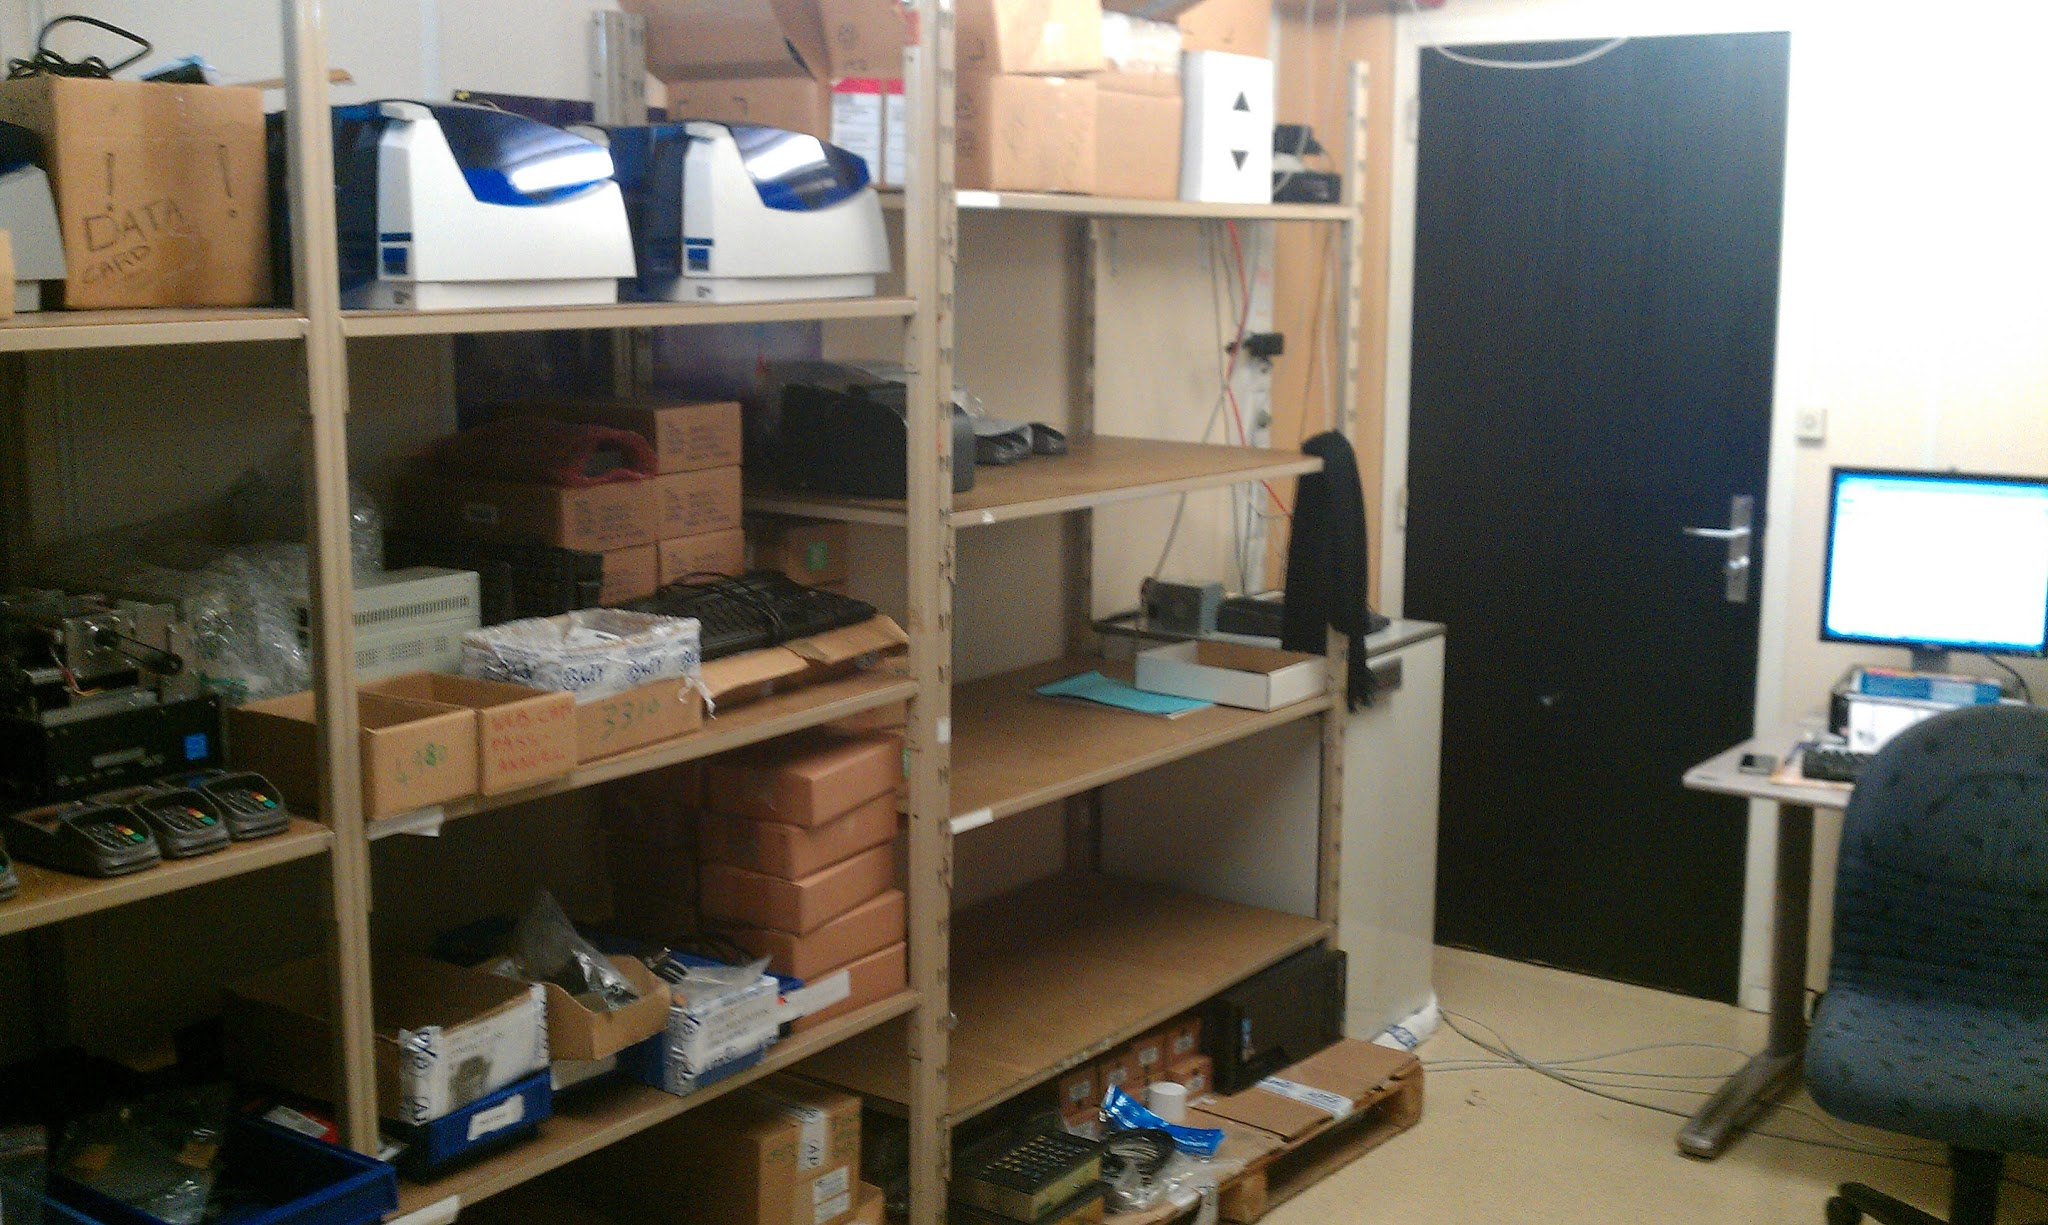
\includegraphics [width=1\textwidth]{images/locaux/IMAG0395.jpg}
  \end{figure}
  \begin{figure}[ht]
    \caption{Les bureaux}
    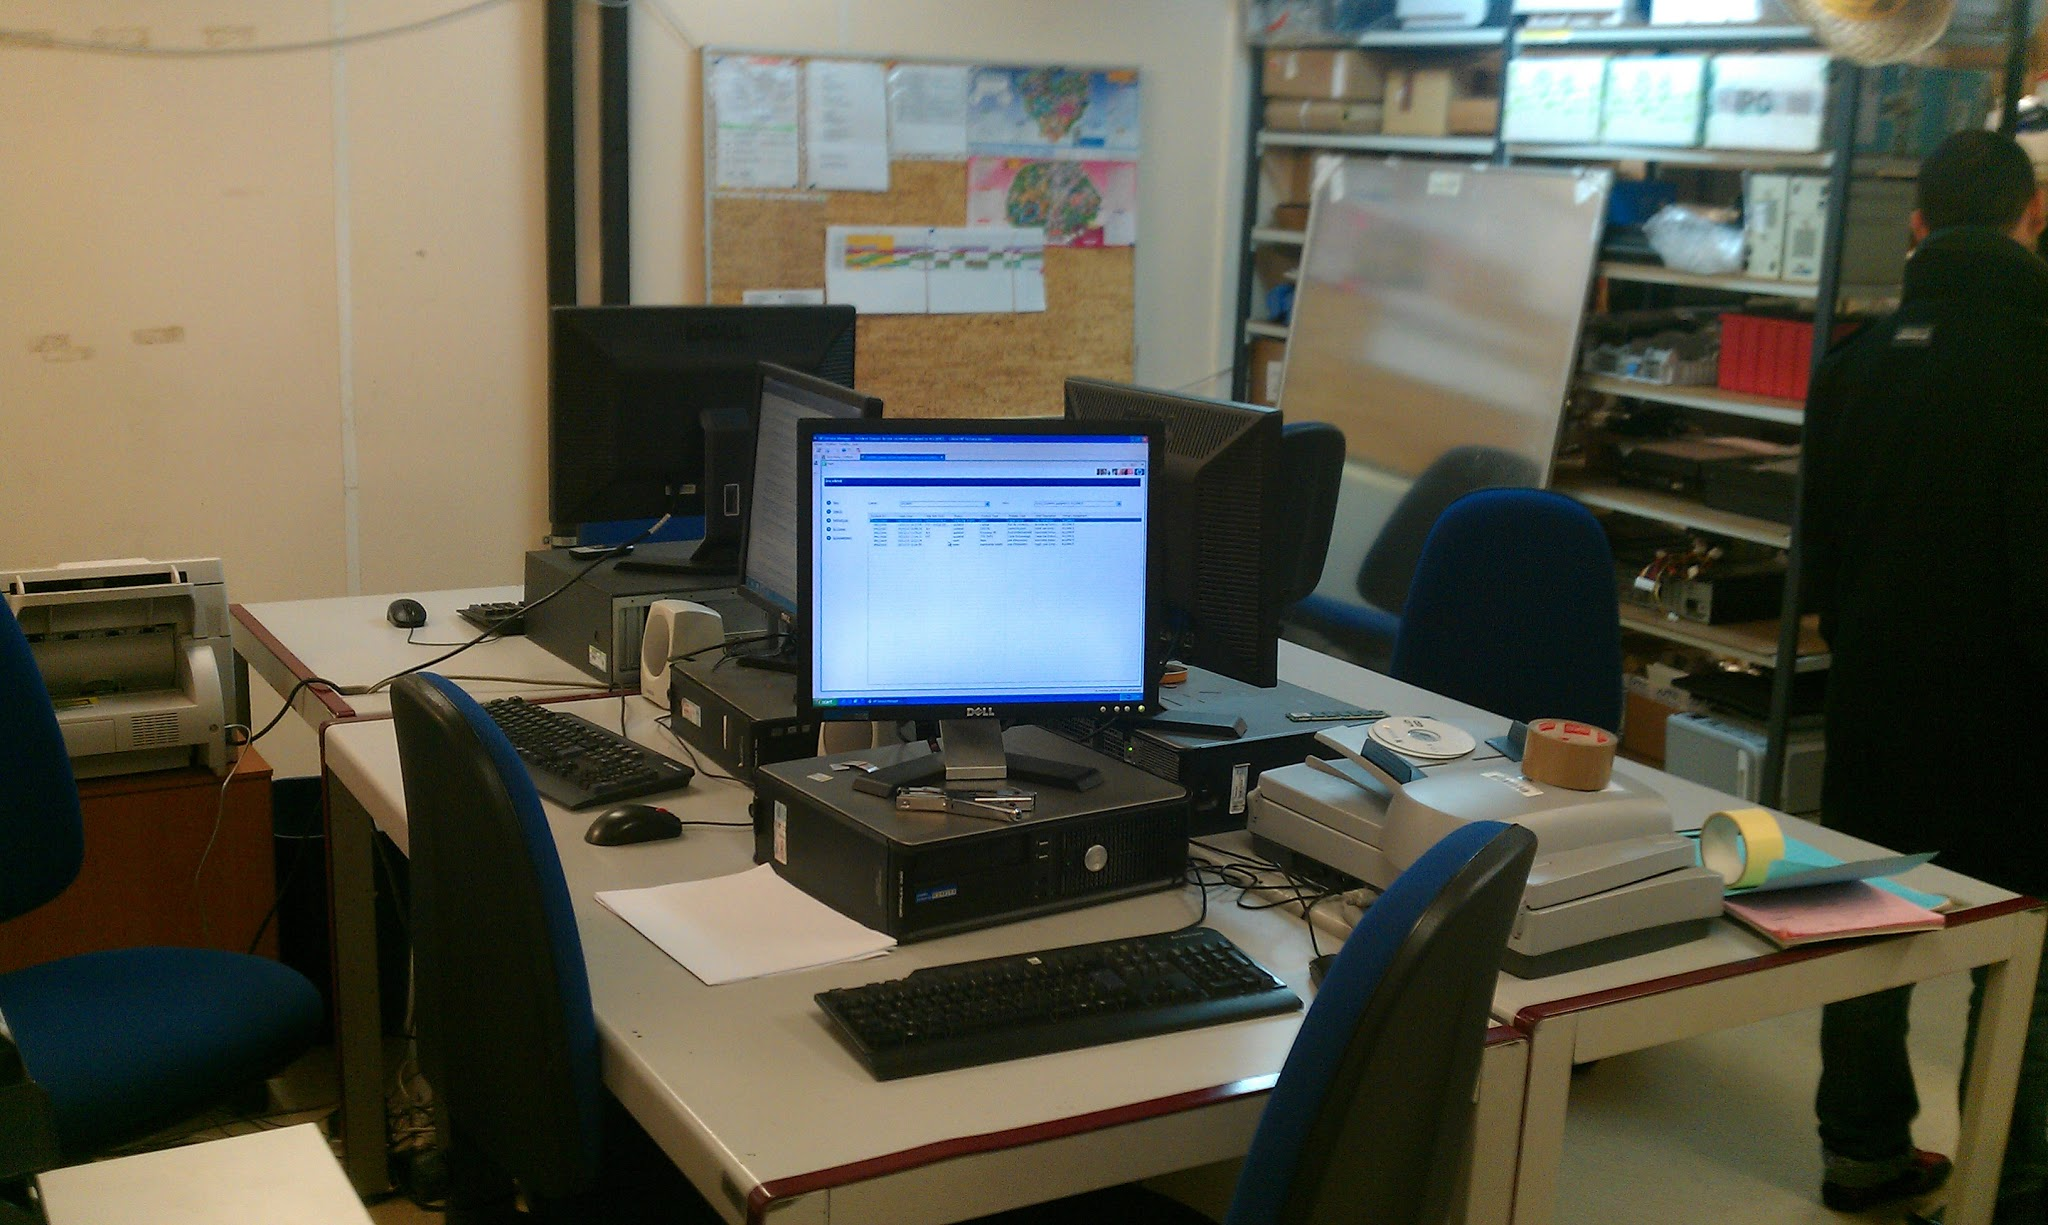
\includegraphics [width=1\textwidth]{images/locaux/IMAG0393.jpg}
  \end{figure}
  \begin{figure}[ht]
    \caption{Les bureaux}
    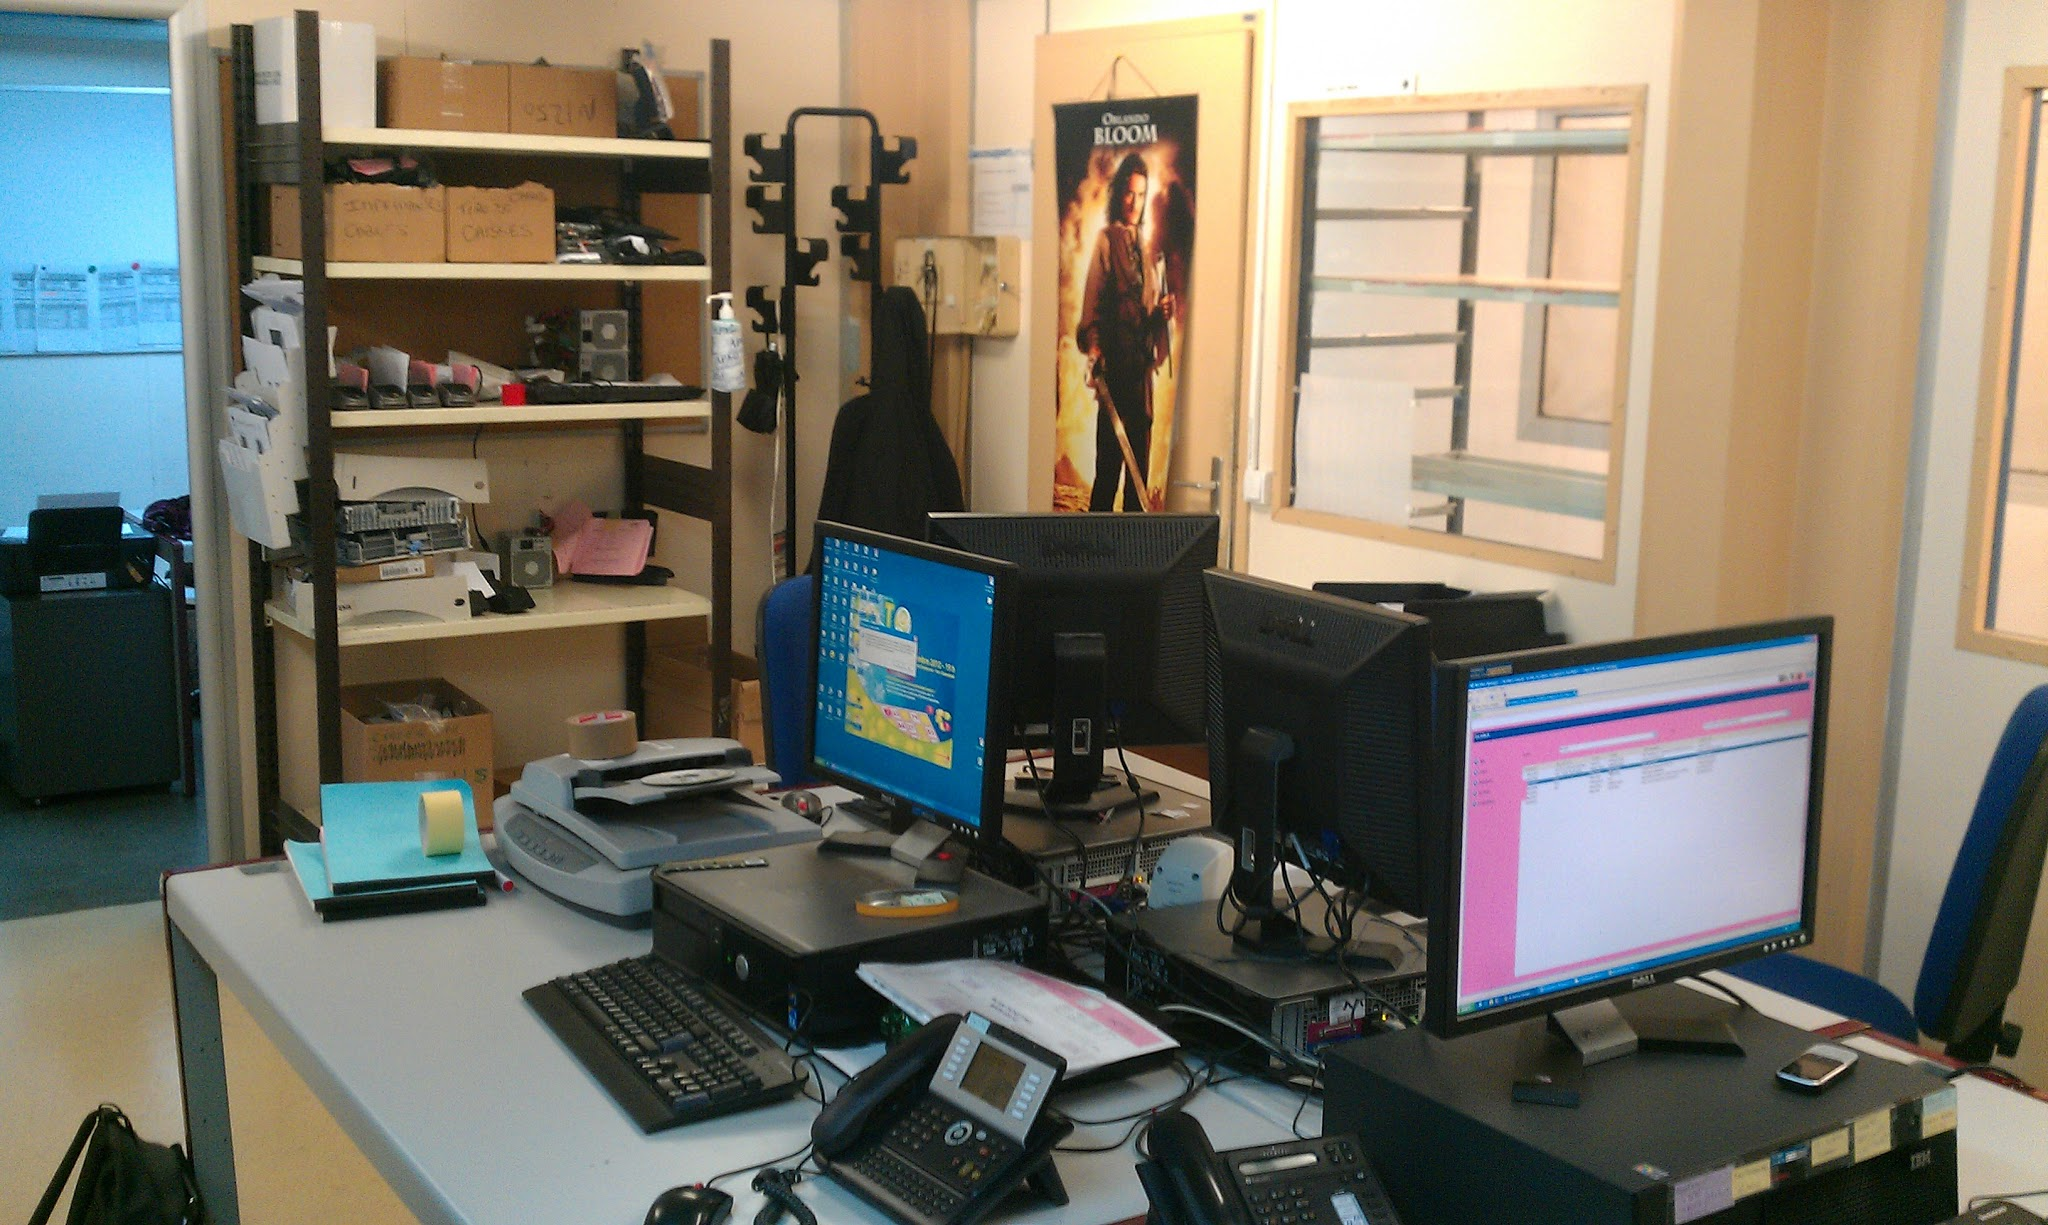
\includegraphics [width=1\textwidth]{images/locaux/IMAG0398.jpg}
  \end{figure}
  \begin{figure}[ht]
    \caption{Le bureau de la chef}
    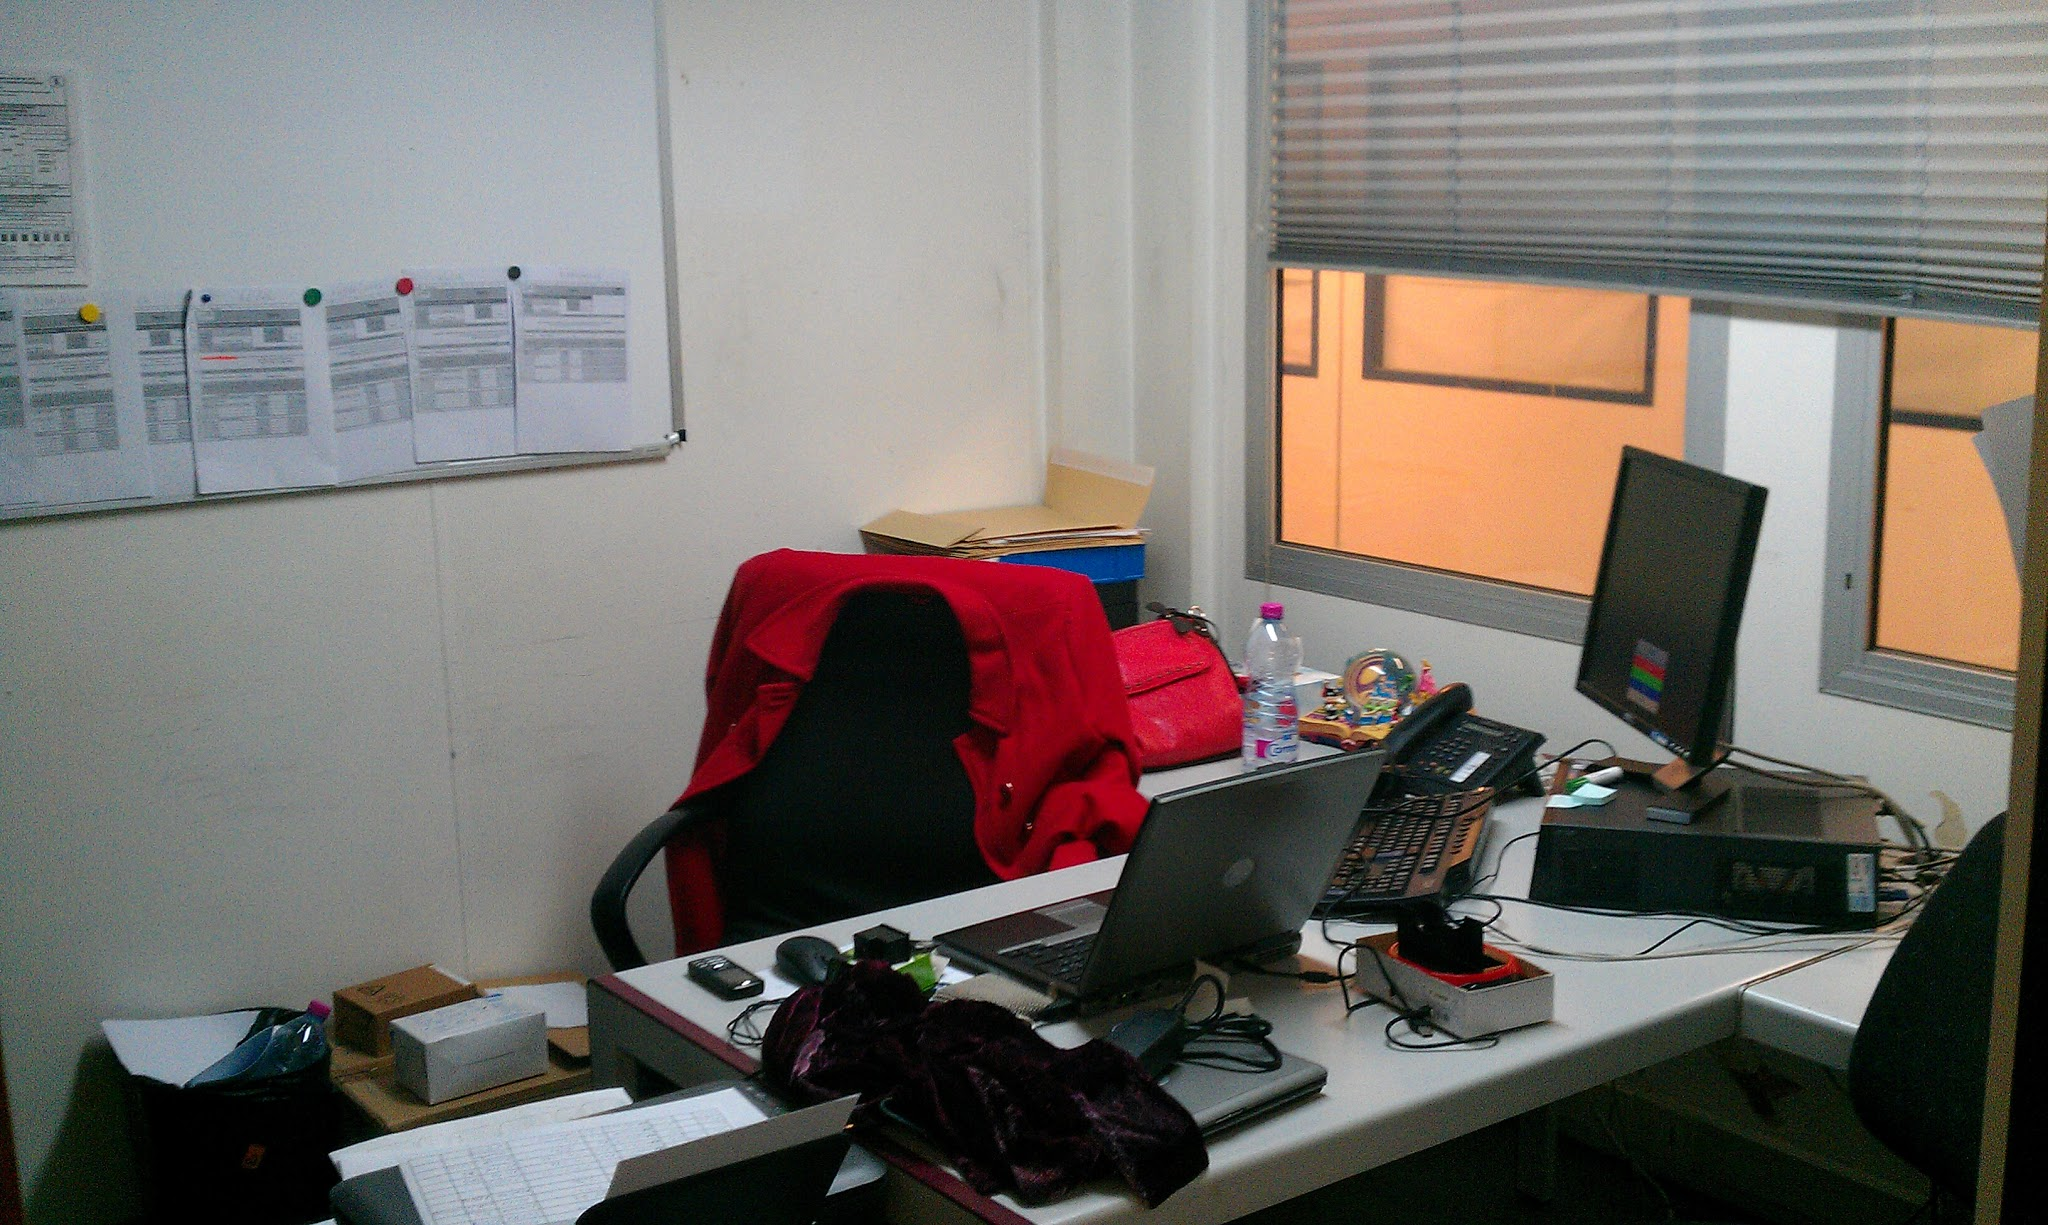
\includegraphics [width=1\textwidth]{images/locaux/IMAG0399.jpg}
  \end{figure}
  \begin{figure}[ht]
    \caption{L'atelier}
    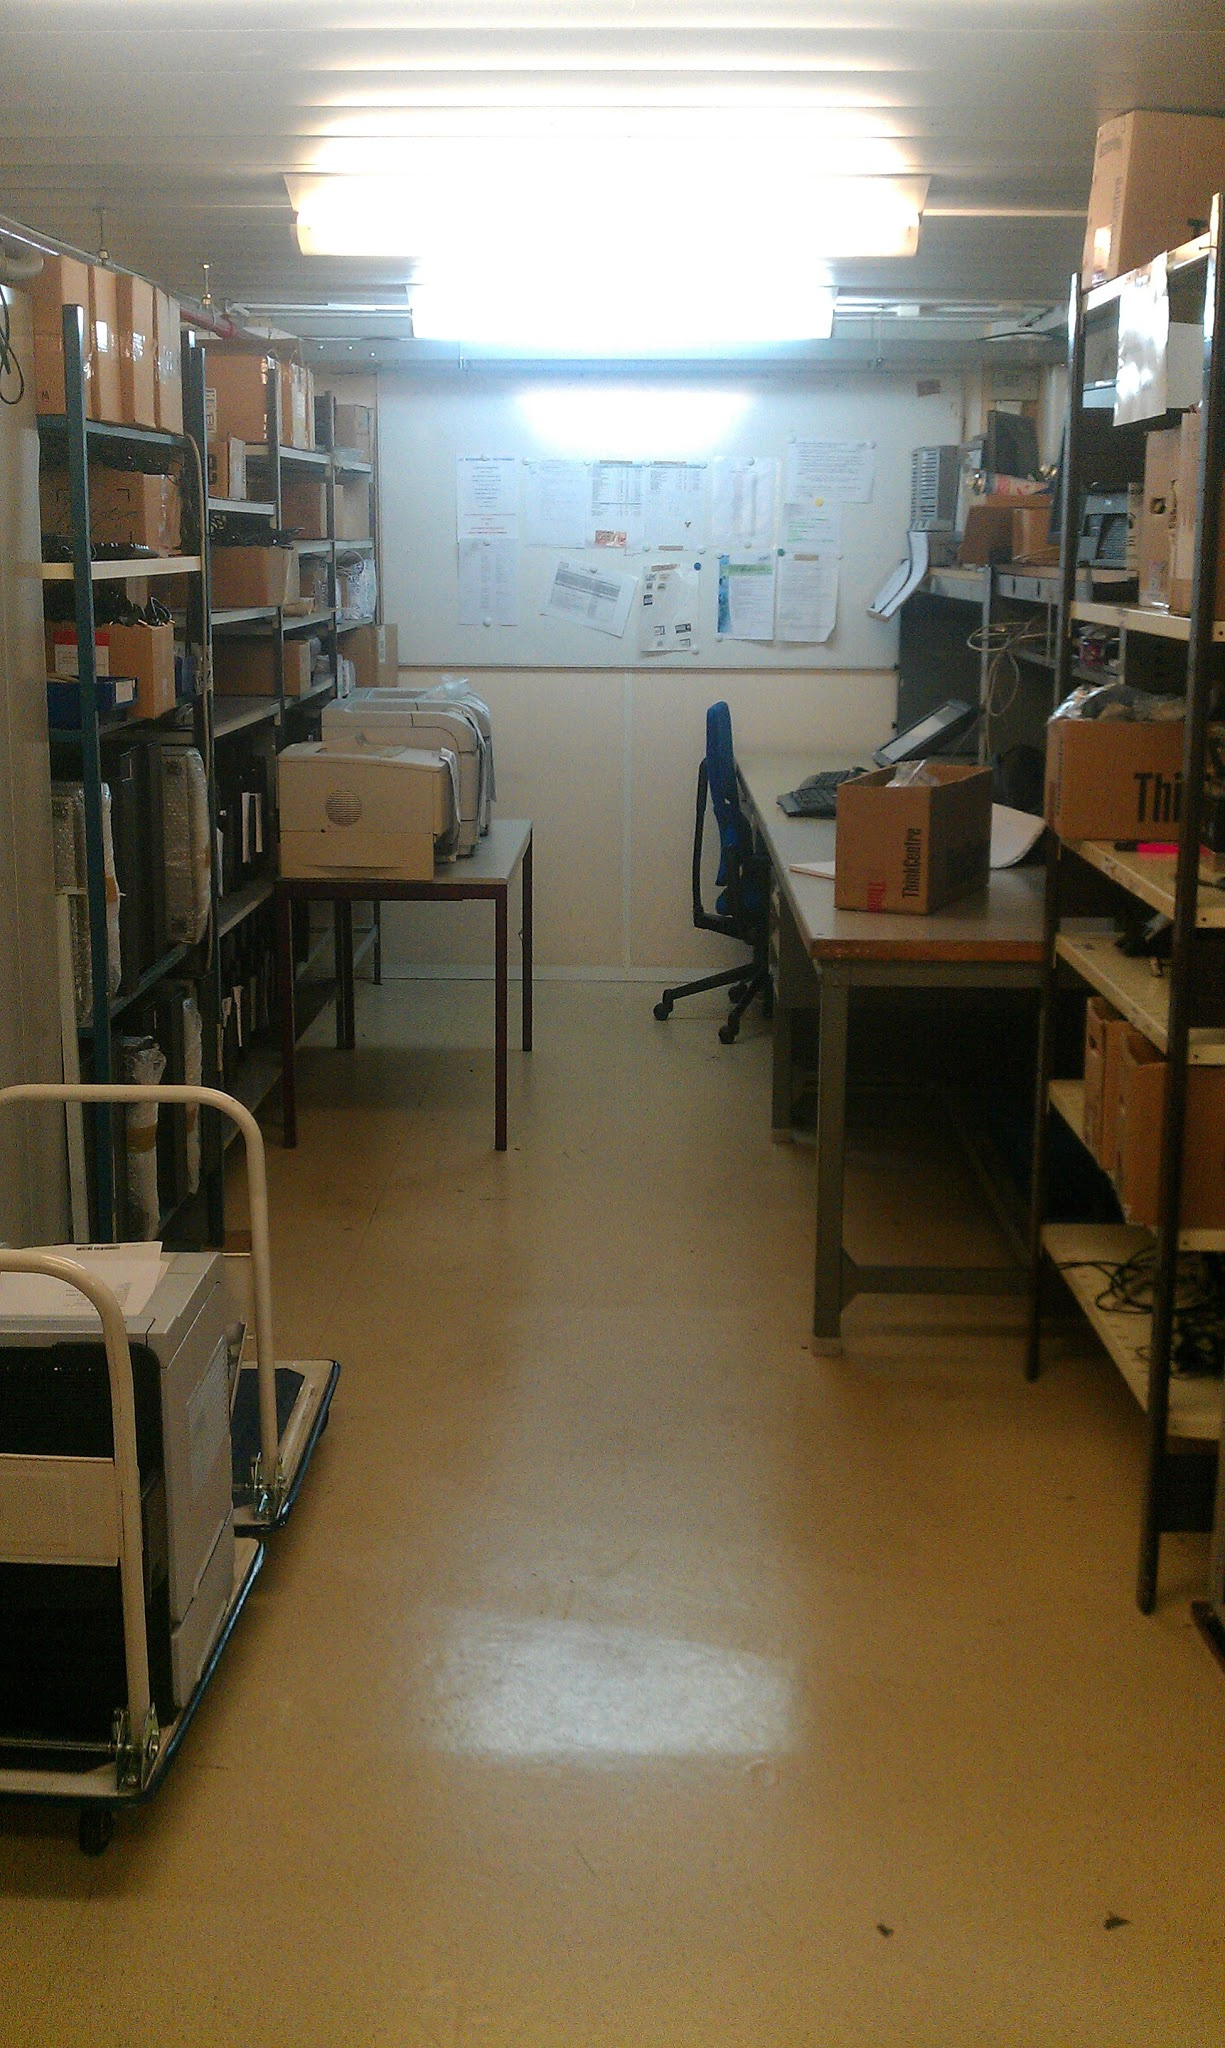
\includegraphics [width=1\textwidth, height=0.8\textheight]{images/locaux/IMAG0400.jpg}
  \end{figure}
\end{center}

\cleardoublepage
\chapter*{SM7}
\addcontentsline{toc}{chapter}{SM7}

\begin{center}
  \begin{figure}[ht]
    \caption{SM7}
    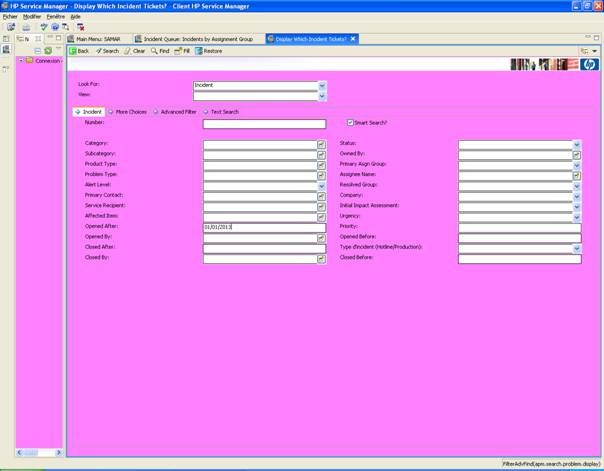
\includegraphics [width=1\textwidth]{images/sm7annexe/image001.jpg}
  \end{figure}
  \begin{figure}[ht]
    \caption{SM7}
    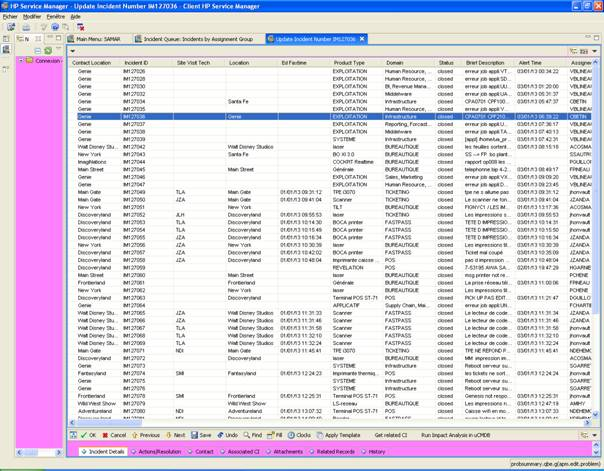
\includegraphics [width=1\textwidth]{images/sm7annexe/image002.jpg}
  \end{figure}
\end{center}

\cleardoublepage
\chapter*{Alloy}
\addcontentsline{toc}{chapter}{Alloy}

\begin{center}
\textbf{Modèle Alloy}
\end{center}
\lstinputlisting[breaklines]{images/alloy/essaiEDTV2.als}



\end{document}
